\documentclass[usenames,dvipsnames,11pt,pdf,utf8,russian,aspectratio=43]{beamer}
\usepackage{cmap}
\usepackage[T2A]{fontenc}
\usepackage[english,russian]{babel}
\usepackage{subfig}
\usepackage{color}
\usepackage{multicol}
\usepackage{appendixnumberbeamer}
\usepackage{multicol}
\usepackage{tikz}
\usepackage{mathbbol}
\usepackage{amssymb}   
\usepackage{xargs}             % AMS Math
\DeclareUnicodeCharacter{00A0}{ } % При наборе текста с планшета появляются невидимые символы. ЭТо костыль.

\DeclareSymbolFontAlphabet{\mathbb}{AMSb}%
\DeclareSymbolFontAlphabet{\amsmathbb}{bbold}%


\usetikzlibrary{arrows,automata}
\usetikzlibrary{positioning}



\DeclareMathOperator*{\argmin}{arg\,min}

\DeclareMathOperator*{\argmax}{arg\,max}
%
% Choose how your presentation looks.
%
% For more themes, color themes and font themes, see:
% http://deic.uab.es/~iblanes/beamer_gallery/index_by_theme.html
%
\mode<presentation>
{
  \usetheme{Boadilla}      % or try Darmstadt, Madrid, Warsaw, ...
  \usecolortheme{seagull} % or try albatross, beaver, crane, ..

  \usefonttheme{structurebold}  % or try serif, structurebold, ...
  \setbeamertemplate{navigation symbols}{}
  \setbeamertemplate{caption}[numbered]

} 
\setbeamercolor{mygray}{fg=gray,bg=white}


\setbeamertemplate{footline}
{
  \leavevmode%
  \hbox{%
  \begin{beamercolorbox}[wd=.9\paperwidth,ht=2.25ex,dp=1ex,center]{}%
   
  \end{beamercolorbox}%
  \begin{beamercolorbox}[wd=.1\paperwidth,ht=2.25ex,dp=1ex]{mygray}%
   
    \insertframenumber{} / \inserttotalframenumber\hspace*{1ex}
  \end{beamercolorbox}}%
  \vskip0pt%
}



\captionsetup[subfloat]{labelformat=empty}
\title[Выбор структуры модели]{Байесовский выбор\\ субоптимальной структуры\\ модели глубокого обучения}
\author{О.\,Ю.\,Бахтеев}


\institute[]{Диссертация на соискание ученой степени\\
кандидата физико-математических наук\\05.13.17 --- Теоретические основы информатики\\Научный руководитель: д.ф.-м.н. В.В. Стрижов\\}     
%\institute[МФТИ]{Московский Физико-Технический Институт (Государственный Университет)}
\date[2019]{Московский физико-технический институт\\6 февраля 2020 г.}
\begin{document}
% nb: очень не люблю макросы. Но что поделать 
% https://stackoverflow.com/questions/1509799/how-to-replace-latex-macros-with-their-definitions-using-latex
\newcommand{\D}{\mathfrak{D}}
\newcommand{\x}{\mathbf{x}}
\newcommand{\X}{\mathbf{X}}
\newcommand{\y}{\mathbf{y}}
\newcommand{\Xb}{\mathbb{X}}
\newcommand{\yb}{\mathbb{Y}}
\newcommand{\F}{\mathfrak{F}}



\newcommand{\w}{\mathbf{w}}
\newcommand{\Wb}{\mathbb{W}}
\newcommand{\Uw}{U_\mathbf{w}}

\newcommand{\Gam}{\boldsymbol{\Gamma}}
\newcommand{\Gb}{\amsmathbb{\Gamma}}
\newcommand{\UG}{U_{\boldsymbol{\Gamma}}}

\newcommand{\h}{\mathbf{h}}
\newcommand{\Hb}{\mathbb{H}}
\newcommand{\Uh}{U_{\mathbf{h}}}

\newcommand{\teta}{\boldsymbol{\theta}}
\newcommand{\Tetab}{\amsmathbb{\Theta}}
\newcommand{\Uteta}{U_{\boldsymbol{\theta}}}

\newcommand{\tetaw}{\boldsymbol{\theta}_\mathbf{w}}
\newcommand{\Tetawb}{\amsmathbb{\Theta}_\mathbf{w}}
\newcommand{\Utetaw}{U_{\boldsymbol{\theta}_\mathbf{w}}}
\newcommand{\tetaG}{\boldsymbol{\theta}_{\boldsymbol{\Gamma}}}
\newcommand{\TetaGb}{\amsmathbb{\Theta}_{\boldsymbol{\Gamma}}}
\newcommand{\UtetaG}{U_{\boldsymbol{\theta}_{\boldsymbol{\Gamma}}}}

\newcommand{\lam}{\boldsymbol{\lambda}}
\newcommand{\Lamb}{\amsmathbb{\Lambda}}
\newcommand{\Ulam}{U_{\boldsymbol{\lambda}}}

%\newcommand{\prior}{p(\mathbf{w}, \boldsymbol{\Gamma}|\mathbf{h},\boldsymbol{\lambda})}
\newcommandx{\prior}[4][1=\mathbf{w},2=\boldsymbol{\Gamma},3=\mathbf{h},4=\boldsymbol{\lambda},usedefault]{p(#1,#2|#3,#4)}
\newcommandx{\priorh}[2][1=\mathbf{h}, 2=\boldsymbol{\lambda},usedefault]{p(#1|#2)}
\newcommandx{\priorG}[3][1=\boldsymbol{\Gamma}, 2= \mathbf{h}, 3=\boldsymbol{\lambda},usedefault]{p(#1|#2,#3)}
\newcommandx{\priorw}[4][1=\mathbf{w},2=\boldsymbol{\Gamma},3=\mathbf{h},4=\boldsymbol{\lambda},usedefault]{p(#1|#2,#3,#4)}


\newcommand{\post}{p(\mathbf{w}, \boldsymbol{\Gamma}|\mathbf{y}, \mathbf{X}, \mathbf{h},\boldsymbol{\lambda})}
\newcommand{\posth}{p(\mathbf{h}|\mathbf{y}, \mathbf{X},\boldsymbol{\lambda})}
\newcommand{\postG}{p(\boldsymbol{\Gamma}|\mathbf{y}, \mathbf{X}, \mathbf{h},\boldsymbol{\lambda})}
\newcommand{\postw}{p(\mathbf{w}|\mathbf{y}, \mathbf{X}, \boldsymbol{\Gamma}, \mathbf{h},\boldsymbol{\lambda})}


\newcommandx{\q}[1][1=\boldsymbol{\theta}, usedefault]{q(\mathbf{w}, \boldsymbol{\Gamma}|#1)}
\newcommandx{\qG}[2][1=\boldsymbol{\Gamma},2=\boldsymbol{\theta}_{\boldsymbol{\Gamma}},usedefault]{q_{\boldsymbol{\Gamma}}(#1|#2)}
\newcommandx{\qw}[3][1=\mathbf{w}, 2=\boldsymbol{\Gamma},3=\boldsymbol{\theta}_\mathbf{w},usedefault]{q_\mathbf{w}(#1|#2,#3)}


\newcommandx{\LL}[4][1=\mathbf{y},2=\mathbf{X},3=\mathbf{w},4=\boldsymbol{\Gamma},usedefault]{p(#1|#2,#3,#4)}

\newcommand{\EV}{p(\mathbf{y}|\mathbf{X}, \mathbf{h},\boldsymbol{\lambda})}

\newcommandx{\Loss}[5][1=\boldsymbol{\theta},2=\mathbf{y},3=\mathbf{X},4=\mathbf{h},5=\boldsymbol{\lambda},usedefault]{L(#1 |#2,#3,#4,#5)}
\newcommandx{\Val}[5][1=\mathbf{h},2=\mathbf{y},3=\mathbf{X},4=\boldsymbol{\theta},5=\boldsymbol{\lambda},usedefault]{Q(#1|#2,#3,#4,#5)}

% прочее
\newcommand{\model}{\mathbf{f}}
\newcommand{\A}{\mathbf{A}}
\newcommand{\s}{\mathbf{s}}
\newcommand{\g}{\boldsymbol{\gamma}}
\newcommand{\E}{\mathsf{E}}
\newcommand{\KL}[2]{D_\text{KL}\bigl(#1 || #2\bigr)}

\newcommand{\lamT}{\lambda_{\text{temp}}}
\newcommand{\lamLL}{\lambda_\text{likelihood}^\text{Q}}
\newcommand{\lamCL}{\lambda_\text{prior}^\text{L}}
\newcommand{\lamCQ}{\lambda_\text{prior}^\text{Q}}
\newcommand{\lamS}{\boldsymbol{\lambda}_\text{struct}^\text{Q}}
\newcommandx{\TLoss}[6][1=\boldsymbol{\theta},2=L,3=\mathbf{y}, 4=\mathbf{X}, 5=\mathbf{h},6=\boldsymbol{\lambda},usedefault]{T(#1|#2,#3,#4,#5,#6)}
\newcommandx{\TVal}[6][1=\mathbf{h},2=Q,3=\mathbf{y}, 4=\mathbf{X}, 5=\boldsymbol{\teta},6=\boldsymbol{\lambda},usedefault]{T(#1|#2,#3,#4,#5,#6)}
%\newcommand{\log}{\text{log}~}




\begin{frame}
  \titlepage
\end{frame}



\begin{frame}{Выбор  структуры модели глубокого обучения}
\small
\textbf{Цель: } предложить метод выбора структуры модели глубокого обучения.\\
\textbf{Задачи}
\begin{enumerate}
\item Предложить критерии оптимальной и субоптимальной сложности модели глубокого обучения.
\item Предложить алгоритм построения модели субоптимальной сложности и оптимизации параметров.
\end{enumerate}
\textbf{Исследуемые проблемы}
\begin{enumerate}
\item Большое число параметров и гиперпараметров модели, высокая вычислительная сложность оптимизации.
\item Многоэкстремальность и невыпуклость задачи оптимизации.
\end{enumerate}
\textbf{Методы исследования}\\ 
Рассматривается графовое представление нейронной сети. Используются методы вариационного байесовского вывода.  Для получения модели субоптимальной сложности используется метод автоматического определения релевантности параметров с использоваением градиентных методов оптимизации гиперпараметров и структурных параметров модели.
\end{frame}



\begin{frame}    
                                                                                                                        
\frametitle{Проблема выбора оптимальной структуры }                                                                                                          
Правдоподобие моделей с избыточным числом параметров значимо не меняется при их удалении.                                                       
\begin{figure}[h]                                                                                                                               
\centering                                                                                                                                      
\subfloat[Избыточность параметров модели]{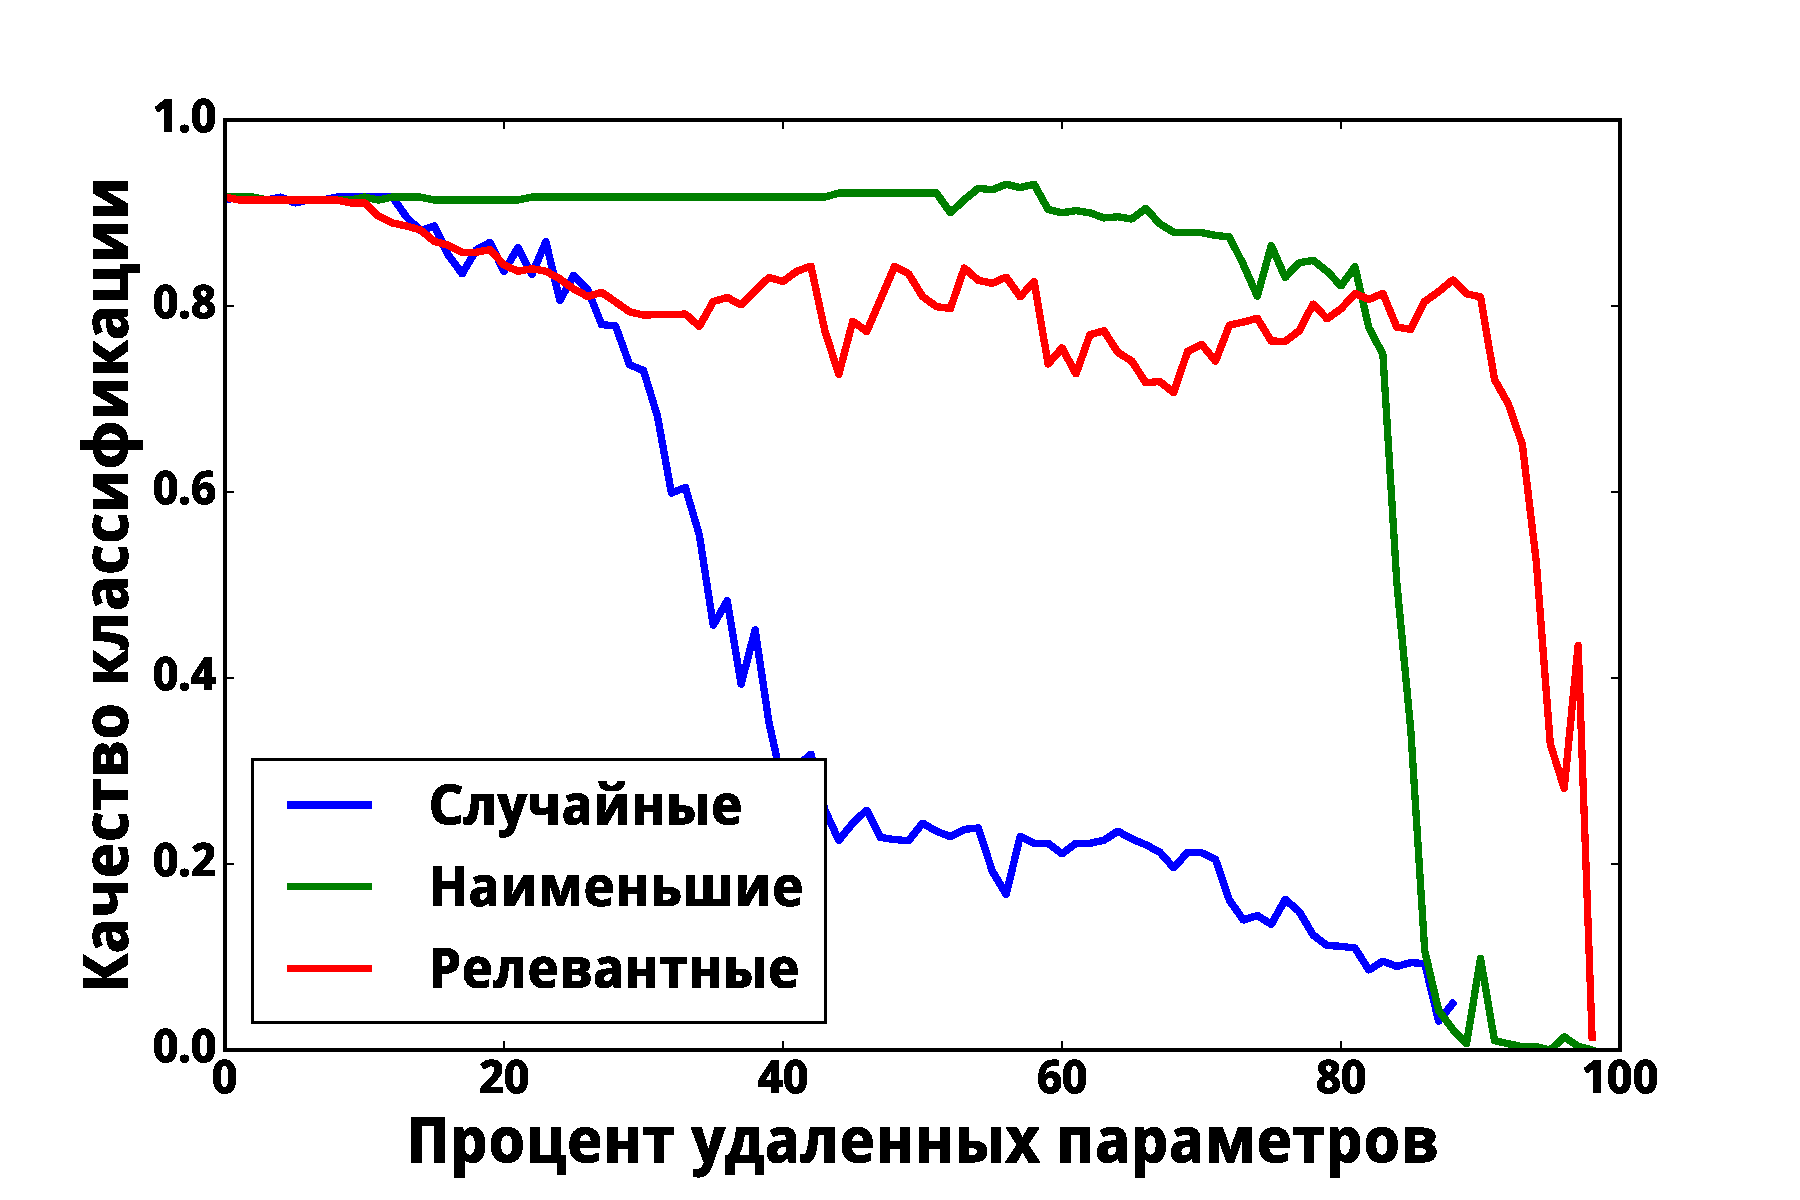
\includegraphics[width=0.55\textwidth]{./slide_plots/pruning.pdf}}   
\hspace*{-1cm}                                       
\subfloat[Устойчивость модели]{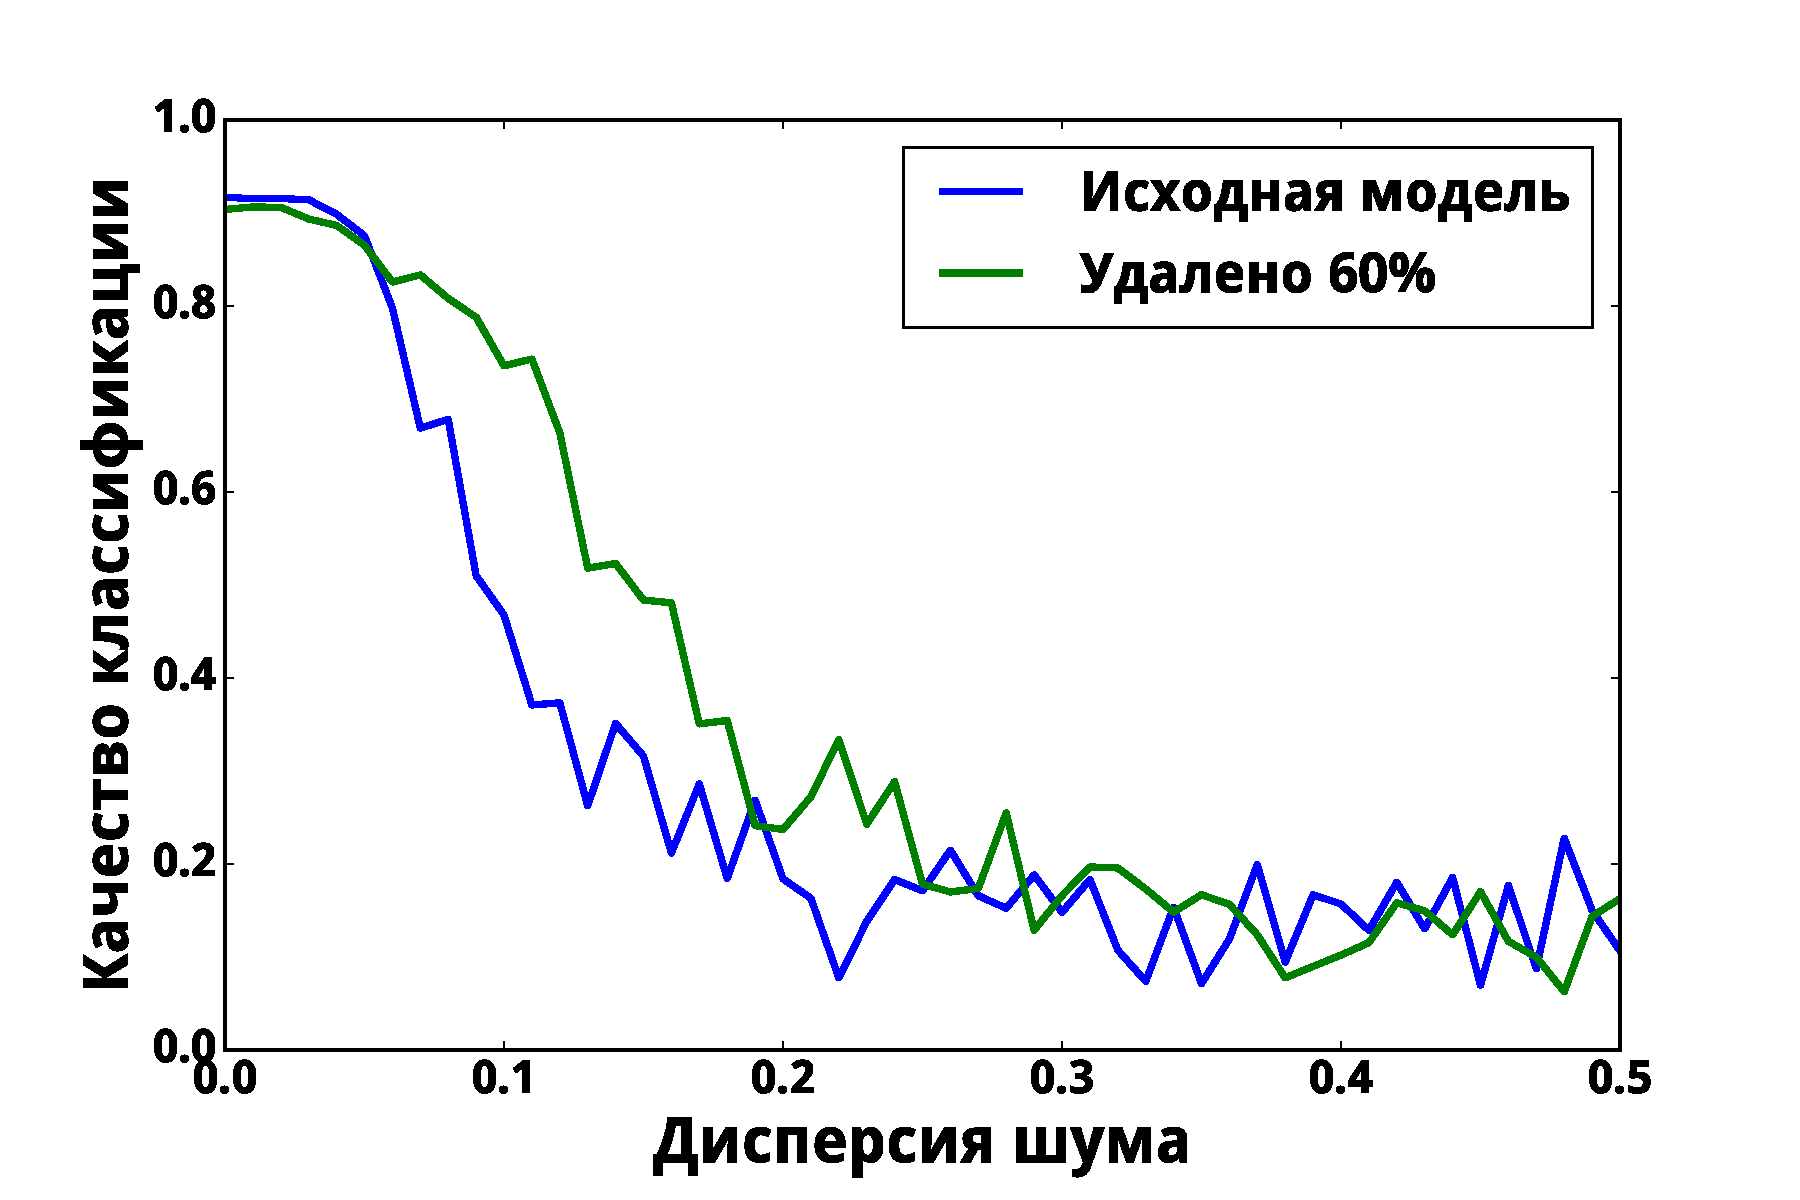
\includegraphics[width=0.55\textwidth]{./slide_plots/noise.pdf}}                                                     
\end{figure}                                                                                                   
\textcolor{gray}{Глубокое обучение предполагает оптимизацию моделей с заведомо избыточной сложностью.}  

                                                                                                                                             
\end{frame}    

\begin{frame}{Модель глубокого обучения}
\small
\begin{block}{Определение}
\textit{Моделью} $\mathbf{f}(\mathbf{w}, \mathbf{x})$ назовем дифференцируемую по параметрам $\mathbf{w}$ функцию из множества признаковых описаний объекта во множество меток:
\[
    \mathbf{f}: \mathbb{X} \times \mathbb{W} \to \mathbb{Y},
\] 
где $\mathbb{W}$ --- пространство параметров функции $\mathbf{f}$.
\end{block}
~\\
\textbf{Особенность задачи}  выбора модели \textit{глубокого обучения} --- значительное число параметров моделей приводит к неприменимости ряда методов оптимизации и выбора структуры модели  (AIC, BIC, кросс-валидация). \\~\\
Модель определяется параметрами $\mathbf{W}$ и структурой $\boldsymbol{\Gamma}$.\\
\textbf{Структура} задает набор суперпозиций, входящих в модель и выбирается согласно статистическим критериям сложности модели.\\

\textbf{Эмпирические оценки статистической сложности модели:}
\begin{enumerate}
\item число параметров;
\item число суперпозиций, из которых состоит модель.
\end{enumerate}
\end{frame}


\begin{frame}{Выбор структуры: двуслойная нейросеть}
\small
Модель $\mathbf{f}$ задана \textbf{структурой}  $\boldsymbol{\Gamma} = [\boldsymbol{\gamma}^{0,1}, {\boldsymbol{\gamma}^{1,2}}].$

\[
    \text{Модель: }\mathbf{f}(\mathbf{x}) = \textbf{softmax}\left((\mathbf{w}^{1,2}_0)^\mathsf{T}{\mathbf{f}_1}(\mathbf{x})\right), \quad \mathbf{f}(\mathbf{x}): \mathbb{R}^n \to [0,1]^{|\mathbb{Y}|}, \quad \mathbf{x} \in \mathbb{R}^n.
\]
\[
\mathbf{f}_1(\mathbf{x}) = {\gamma}^{0,1}_{0}\mathbf{g}^{0,1}_{0}(\mathbf{x}) + {\gamma}^{0,1}_{1}\mathbf{g}^{0,1}_{1}(\mathbf{x}),
\]
где $\mathbf{w} = [\mathbf{w}^{0,1}_0, \mathbf{w}^{0,1}_1, \mathbf{w}^{1,2}_0]^{\text{T}}$ --- матрицы параметров, $\{\mathbf{g}_{0}^{0,1},\mathbf{g}_{1}^{0,1},{\mathbf{g}_{0}^{1,2}\}}$ --- обобщенно-линейные функции скрытых слоев нейросети.

\begin{tikzpicture}[node distance=0.5cm, auto]
  %\tikzstyle{every state}=[fill=red,draw=none,text=white]

  \node (f0)  at (1,6)                  {$\mathbf{f}_0(\mathbf{x}) = \mathbf{x}$};
  %\node (g11) at (6,3)                    {$\mathbf{g}^{1,1}(\mathbf{x})$};% = \text{Conv}(\mathbf{x}, 3, 32, 1)$};
  %\node (g12)  at (6,9)                   {$\mathbf{g}^{1,2}(\mathbf{x})$};% = \text{Conv}(\mathbf{x}, 4, 32, 1)$};
  \node (f1)  at (7,6)                 {$\mathbf{f}_1(\mathbf{x})$};% = \gamma^{1,1}\mathbf{g}^{1,1}(\mathbf{x}) +  \gamma^{1,2}\mathbf{g}^{1,2}(\mathbf{x})$};
  %\node (g21) at (12,6)                   {$\mathbf{g}^{2,1}(\mathbf{x})$};% = \boldsymbol{\sigma}(\mathbf{w}^{2,1}\mathbf{x})$};
  \node (f2)  at (12,6)                   {$\mathbf{f}_2(\mathbf{x})$};% = \gamma^{2,1}\mathbf{g}^{2,1}(\mathbf{x})$};
  \path[->]  (f0) edge [bend left=50] node {$\gamma^{0,1}_0\mathbf{g}^{0,1}_0(\mathbf{x}) = \gamma^{0,1}_0\boldsymbol{\sigma}\left((\mathbf{w}^{0,1}_0)^{\mathsf{T}}\mathbf{x}\right)$}(f1);
  \path[->] (f0)  edge[bend right=50] node[below] {$\gamma^{0,1}_1\mathbf{g}^{0,1}_1(\mathbf{x}) = \gamma^{0,1}_1\boldsymbol{\sigma}\left((\mathbf{w}^{0,1}_1)^{\mathsf{T}}\mathbf{x}\right)$}(f1);
  \path[->] (f1)  edge node {$\gamma^{1,2}_0\mathbf{g}^{1,2}_0(\mathbf{x}) = \gamma^{1,2}_0\textbf{softmax}\left((\mathbf{w}^{1,2}_0)^{\mathsf{T}}\mathbf{x}\right)$}(f2);       
  \draw[->] (f1) to (f2);
 
\end{tikzpicture}

\end{frame}


\begin{frame}{Графовое представление модели глубокого обучения}
\footnotesize
Заданы:
\begin{enumerate}
 \item ациклический граф $(V,E)$;
\item для каждого ребра $(j,k) \in E$: вектор базовых дифференцируемых функций  $\mathbf{g}^{j,k} = [\mathbf{g}^{j,k}_0, \dots, \mathbf{g}^{j,k}_{K^{j,k}}]$  мощности $K^{j,k}$;
\item для каждой вершины $v \in V$: дифференцируемая функция агрегации $\textbf{agg}_v$.
\item Функция $\mathbf{f} = \mathbf{f}_{|V|-1}$, задаваемая по правилу 
\begin{equation}
\label{eq:modelfam}
    \mathbf{f}_{v}(\mathbf{w}, \mathbf{x}) = \textbf{agg}_{v}\left(\{ \langle \boldsymbol{\gamma}^{j,k}, \mathbf{g}^{j,k} \rangle \circ  \mathbf{f}_j(\mathbf{x})| j \in \text{Adj}(v_k)\}\right), v \in \{1,\dots,|V|-1\}, \quad \mathbf{f}_0(\mathbf{x}) = \mathbf{x}
\end{equation}
и являющаяся функцией из признакового пространства $\mathbb{X}$ в пространство меток $\mathbb{Y}$ при значениях векторов, $\boldsymbol{\gamma}^{j,k} \in [0,1]^{K^{j,k}}$.
\end{enumerate}

\begin{block}{Определение}
Граф $(V, E)$ со множестом векторов базовых функций $\{\mathbf{g}^{j,k}, (j,k) \in E\}$ и функций агрегаций $\{ \textbf{agg}_v, {v \in V}\}$ назовем \textit{параметрическим семейством моделей} $\mathfrak{F}$.
\end{block}
\begin{block}{Утверждение}
Для любого значения $\boldsymbol{\gamma}^{j,k} \in [0,1]^{K^{j,k}}$ функция $\mathbf{f} \in \mathfrak{F}$ является моделью.
\end{block}
\end{frame}

      

\begin{frame}{Ограничения на структурные параметры}
Примеры ограничений для одного структурного параметра $\boldsymbol{\gamma}, |\boldsymbol{\gamma}| = 3$.
\begin{figure}
 \begin{minipage}[t]{.45\textwidth}
        \centering
%1 limit
\begin{tikzpicture}[%
x={(1.5cm,0cm)},
y={(0cm,1.5cm)},
z={({0.5*cos(45)},{0.5*sin(45)})},
]

\coordinate (A) at (0,0,0); 
\coordinate (B) at (1,0,0) ;
\coordinate (C) at (1,1,0); 
\coordinate (D) at (0,1,0); 
\coordinate (E) at (0,0,1); 
\coordinate (F) at (1,0,1); 
\coordinate (G) at (1,1,1); 
\coordinate (H) at (0,1,1   );

%Ecken
\node[circle,scale=0.5,fill=black,draw=black](Ap) at (0,0,0){};
\node[circle,scale=0.5,fill=black,draw=black](Bp) at (1,0,0){};
\node[circle,scale=0.5,fill=black,draw=black](Cp) at (1,1,0){};
\node[circle,scale=0.5,fill=black,draw=black](Dp) at (0,1,0){};
\node[circle,scale=0.5,fill=black,draw=black](Ep) at (0,0,1){};
\node[circle,scale=0.5,fill=black,draw=black](Fp) at (1,0,1){};
\node[circle,scale=0.5,fill=black,draw=black](Gp) at (1,1,1){};
\node[circle,scale=0.5,fill=black,draw=black](Hp) at (0,1,1){};
\node[left= 1pt of A]{[0,0,0]};
\node[right= 1pt of B]{[1,0,0]};
\node[right= 1pt of C]{[1,1,0]};
\node[left= 1pt of D]{[0,1,0]};
\node[left= 1pt of E]{[0,0,1]};
\node[right= 1pt of F]{[1,0,1]};
\node[right= 1pt of G]{[1,1,1]};
\node[left= 1pt of H]{[0,1,1]};

%Kanten
\draw[] (A)
-- (B)  node[midway, below]{}
-- (C)      node[midway, right]{}
-- (D)  node[midway, above]{}
-- (A)  node[midway, left]{};
\draw[] (B) -- (F) -- (G) -- (C);
\draw[] (G) -- (H) -- (D);
\draw[densely dashed] (A) -- (E) -- (F);
\draw[densely dashed] (E) -- (H);

\end{tikzpicture}
\caption*{На вершинах куба}
\end{minipage}
\hfill
 \begin{minipage}[t]{.45\textwidth}
        \centering

%2 limit
\begin{tikzpicture}[%
x={(1.5cm,0cm)},
y={(0cm,1.5cm)},
z={({0.5*cos(45)},{0.5*sin(45)})},
]

\coordinate (A) at (0,0,0); 
\coordinate (B) at (1,0,0) ;
\coordinate (C) at (1,1,0); 
\coordinate (D) at (0,1,0); 
\coordinate (E) at (0,0,1); 
\coordinate (F) at (1,0,1); 
\coordinate (G) at (1,1,1); 
\coordinate (H) at (0,1,1   );

%Ecken
\node[left= 1pt of A]{[0,0,0]};
\node[right= 1pt of B]{[1,0,0]};
\node[right= 1pt of C]{};
\node[left= 1pt of D]{[0,1,0]};
\node[left= 1pt of E]{};
\node[right= 1pt of F]{[1,0,1]};
\node[right= 1pt of G]{[1,1,1]};
\node[left= 1pt of H]{[0,1,1]};

%Kanten
\draw[fill=gray] (A)
-- (B)  node[midway, below]{}
-- (C)      node[midway, right]{}
-- (D)  node[midway, above]{}
-- (A)  node[midway, left]{};
\draw[fill=gray] (B) -- (F) -- (G) -- (C);
\draw[fill=gray] (G) -- (H) -- (D);
\draw[fill=gray] (A) -- (E) -- (F);
\draw[fill=gray] (E) -- (H);
\draw[fill=gray] (D) -- (H) -- (G) -- (C);
\end{tikzpicture}
\caption*{Внутри куба}
\end{minipage}
\hfill
 \begin{minipage}[t]{.45\textwidth}
        \centering
%3 limit
\begin{tikzpicture}[%
x={(1.5cm,0cm)},
y={(0cm,1.5cm)},
z={({0.5*cos(45)},{0.5*sin(45)})},
]

\coordinate (A) at (0,0,0); 
\coordinate (B) at (1,0,0) ;
\coordinate (C) at (1,1,0); 
\coordinate (D) at (0,1,0); 
\coordinate (E) at (0,0,1); 
\coordinate (F) at (1,0,1); 
\coordinate (G) at (1,1,1); 
\coordinate (H) at (0,1,1   );

%Ecken
\node[circle,scale=0.5,fill=black,draw=black](Bp) at (1,0,0){};
\node[circle,scale=0.5,fill=black,draw=black](Dp) at (0,1,0){};
\node[circle,scale=0.5,fill=black,draw=black](Ep) at (0,0,1){};
\node[left= 1pt of A]{};
\node[right= 1pt of B]{[1,0,0]};
\node[right= 1pt of C]{};
\node[left= 1pt of D]{[0,1,0]};
\node[left= 1pt of E]{[0,0,1]};
\node[right= 1pt of F]{};
\node[right= 1pt of G]{};
\node[left= 1pt of H]{};

%Kanten
\draw[] (A)
-- (B)  node[midway, below]{}
-- (C)      node[midway, right]{}
-- (D)  node[midway, above]{}
-- (A)  node[midway, left]{};
\draw[] (B) -- (F) -- (G) -- (C);
\draw[] (G) -- (H) -- (D);
\draw[densely dashed] (A) -- (E) -- (F);
\draw[densely dashed] (E) -- (H);

\end{tikzpicture}
\caption*{На вершинах симплекса}
\end{minipage}
\hfill
 \begin{minipage}[t]{.45\textwidth}
        \centering
%4 limit
\begin{tikzpicture}[%
x={(1.5cm,0cm)},
y={(0cm,1.5cm)},
z={({0.5*cos(45)},{0.5*sin(45)})},
]

\coordinate (A) at (0,0,0); 
\coordinate (B) at (1,0,0) ;
\coordinate (C) at (1,1,0); 
\coordinate (D) at (0,1,0); 
\coordinate (E) at (0,0,1); 
\coordinate (F) at (1,0,1); 
\coordinate (G) at (1,1,1); 
\coordinate (H) at (0,1,1   );

%Ecken
\node[left= 1pt of A]{};
\node[right= 1pt of B]{[1,0,0]};
\node[right= 1pt of C]{};
\node[left= 1pt of D]{[0,1,0]};
\node[left= 1pt of E]{[0,0,1]};
\node[right= 1pt of F]{};
\node[right= 1pt of G]{};
\node[left= 1pt of H]{};

%Kanten
\draw[] (A)
-- (B)  node[midway, below]{}
-- (C)      node[midway, right]{}
-- (D)  node[midway, above]{}
-- (A)  node[midway, left]{};
\draw[] (B) -- (F) -- (G) -- (C);
\draw[] (G) -- (H) -- (D);
\draw[densely dashed] (A) -- (E) -- (F);
\draw[densely dashed] (E) -- (H);
\draw[fill=gray] (B) -- (D) -- (E);


\end{tikzpicture}
\caption*{Внутри симплекса}
\end{minipage}

\end{figure}

\end{frame}






\begin{frame}{Априорное распределение параметров}
\footnotesize   
\begin{columns}
\begin{column}{0.6\textwidth}
   \begin{block}{Определение}
\textit{Априорным распределением} параметров $\mathbf{w}$ и структуры  $\boldsymbol{\Gamma}$ модели $\mathbf{f}$ назовем вероятностное распределение
$
    \textcolor{red}{p(\mathbf{W}, \boldsymbol{\Gamma}|\mathbf{h},\lam)}: \mathbb{W} \times \amsmathbb{\Gamma} \times \mathbb{H} \to \mathbb{R}^{+}, 
$
где $\mathbb{W}$ --- множество значений параметров модели, $\amsmathbb{\Gamma}$~---~множество значений структуры модели.
\end{block}

\end{column}
\begin{column}{0.4\textwidth}  %%<--- here
    \begin{center}
     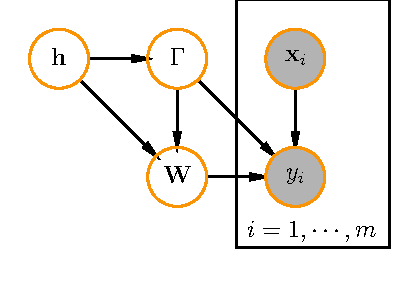
\includegraphics[width=\textwidth]{simple_plate.pdf}
     \end{center}
\end{column}
\end{columns}
\vspace*{-0.5cm}
\begin{block}{Определение}
\textit{Гиперпараметрами} $\mathbf{h}\in \mathbb{H}$ модели  назовем параметры распределения $p(\mathbf{w}, \boldsymbol{\Gamma}|\mathbf{h},\mathbf{f})$ (параметры распределения параметров модели $\mathbf{f}$).
 
\end{block}
Модель $\mathbf{f}$ задается следующими величинами:
\begin{itemize}
\item \textbf{Параметры} $\mathbf{w} \in \mathbb{W}$ задают суперпозиции $\mathbf{f}_v$, из которых состоит модель $\mathbf{f}$.
\item \textbf{Структурные параметры} $\boldsymbol{\Gamma}=\{\gamma^{j,k}\}_{(j,k)\in E} \in \amsmathbb{\Gamma}$ задают вклад суперпозиций $\mathbf{f}_v$ в модель $\mathbf{f}$.
\item \textbf{Гиперпараметры} $\mathbf{h} \in \mathbb{H}$ задают распределение параметров и структурных параметров модели.
\item \textbf{Метапараметры} $\boldsymbol{\lambda} \in \amsmathbb{\Lambda}$ задают вид оптимизации модели.
\end{itemize}

\end{frame}






\begin{frame}{Априорное распределение на структуре модели}
Каждая точка на симплексе задает модель.


\textbf{Распределение Гумбель-софтмакс: }$\textcolor{red}{\boldsymbol{\Gamma}\sim \text{GS}(\mathbf{s}, \lambda_\text{temp})}$\\
\begin{figure}
 \begin{minipage}[t]{.3\textwidth}
        \centering
\begin{tikzpicture}[%
x={(1.7cm,0cm)},
y={(0cm,1.7cm)},
]

\coordinate (A) at (0,0); 
\coordinate (B) at (1,0) ;
\coordinate (C) at (0.5,0.86); 

%Ecken
\node[circle,scale=0.5,fill=black,draw=black](Ap) at (0,0){};
\node[circle,scale=0.5,fill=black,draw=black](Bp) at (1,0){};
\node[circle,scale=0.5,fill=black,draw=black](Cp) at (0.5,0.86){};

%Kanten
\draw[] (A)
-- (B)  node[midway, below]{}
-- (C)      node[midway, right]{}
-- (A)  node[midway, left]{};

\end{tikzpicture}
\caption*{$\lambda_\text{temp}\to0$}
\end{minipage}
\hfill
 \begin{minipage}[t]{.3\textwidth}
   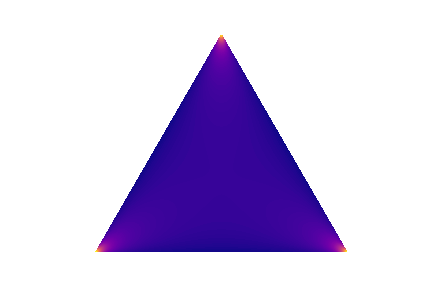
\includegraphics[width=\textwidth]{gs0995.png}
\caption*{$\lambda_\text{temp}=0.995$}
\end{minipage}
\hfill
 \begin{minipage}[t]{.3\textwidth}
   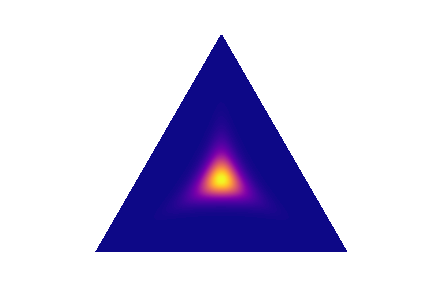
\includegraphics[width=\textwidth]{gs5.png}
\caption*{$\lambda_\text{temp}=5.0$}
\end{minipage}

\end{figure}

\textbf{Распределение Дирихле: }$\textcolor{red}{\boldsymbol{\Gamma}\sim \text{Dir}(\mathbf{s}, \lambda_\text{temp})}$\\
\begin{figure}
 \begin{minipage}[t]{.3\textwidth}
        \centering
\begin{tikzpicture}[%
x={(1.7cm,0cm)},
y={(0cm,1.7cm)},
]

\coordinate (A) at (0,0); 
\coordinate (B) at (1,0) ;
\coordinate (C) at (0.5,0.86); 

%Ecken
\node[circle,scale=0.5,fill=black,draw=black](Ap) at (0,0){};
\node[circle,scale=0.5,fill=black,draw=black](Bp) at (1,0){};
\node[circle,scale=0.5,fill=black,draw=black](Cp) at (0.5,0.86){};

%Kanten
\draw[] (A)
-- (B)  node[midway, below]{}
-- (C)      node[midway, right]{}
-- (A)  node[midway, left]{};

\end{tikzpicture}
\caption*{$\lambda_\text{temp}\to0$}
\end{minipage}
\hfill
 \begin{minipage}[t]{.3\textwidth}
   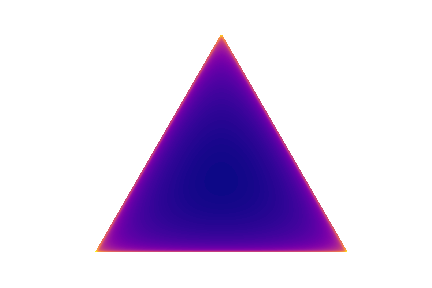
\includegraphics[width=\textwidth]{dir0995.png}
\caption*{$\lambda_\text{temp}=0.995$}
\end{minipage}
\hfill
 \begin{minipage}[t]{.3\textwidth}
   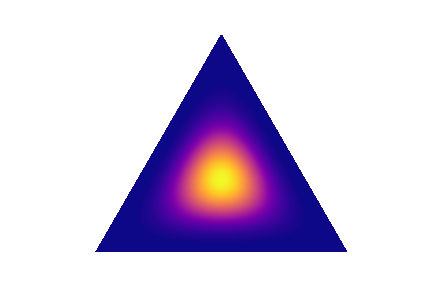
\includegraphics[width=\textwidth]{dir5.png}
\caption*{$\lambda_\text{temp}=5.0$}
\end{minipage}

\end{figure}

\end{frame}


\begin{frame}{Байесовский выбор модели}


\begin{columns}
\begin{column}{0.4\textwidth}
\textbf{Базовая модель:} %https://www.microsoft.com/en-us/research/wp-content/uploads/2016/02/bishop-variational-icann-98.pdf
\begin{itemize}
\item \textbf{параметры} модели\\ $\textcolor{red}{\mathbf{w} \sim \mathcal{N}(0, \alpha^{-1})},$
\item \textbf{гиперпараметры} модели $\mathbf{h} = [\alpha].$
\end{itemize}
\begin{figure}
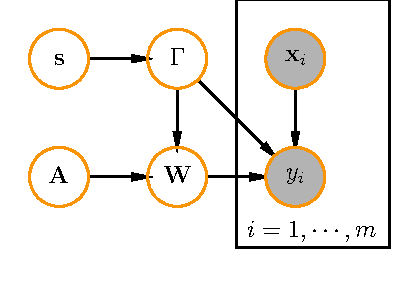
\includegraphics[width=\textwidth]{simple_plate_concrete.pdf}
\end{figure}
\end{column}
\begin{column}{0.6\textwidth}
\textbf{Предлагаемая модель: }
\begin{itemize}
\item \textbf{параметры} модели\\ $\textcolor{red}{\mathbf{w}_r^{j,k} \sim \mathcal{N}(0, (\gamma_{r}^{j,k})^2 (\mathbf{A}_r^{j,k})^{-1})},$
$\mathbf{A}_r^{j,k}$ --- диагональная матрица параметров, соответствующих базовых функций $\mathbf{g}_r^{j,k}$,
\\$\textcolor{OliveGreen}{(\mathbf{A}_r^{j,k})^{-1} \sim \text{inv-gamma}(\lambda_1,\lambda_2)},$

\item \textbf{структурные параметры} модели \\$\boldsymbol{\Gamma} = \{\boldsymbol{\gamma}^{j,k}, (j,k) \in E\},$ \\$\textcolor{red}{\boldsymbol{\gamma}^{j,k} \sim \text{GS}(\mathbf{s}^{j,k}, \lambda_\text{temp})},$ 
\item \textbf{гиперпараметры} модели $\mathbf{h} = [\text{diag}(\mathbf{A}), \mathbf{s} ],$
\item \textbf{метапараметры} $\lambda_1,\lambda_2,\lambda_\text{temp}$.
\end{itemize}

\end{column}

\end{columns}

%

\end{frame}


\begin{frame}{Обоснованность как статистическая сложность}  
\footnotesize
\textbf{Статистическая сложность} модели $\mathbf{f}$:
\[
	\text{MDL}(\mathbf{y},\mathbf{f}) = \textcolor{OliveGreen}{-\text{log}~p(\mathbf{h}|\mathbf{f})} - \textcolor{red}{\text{log}~p(\hat{\mathbf{w}} | \mathbf{h},\mathbf{f})}-  \textcolor{blue}{\text{log}~\bigl(p(\mathbf{y}|\mathbf{X}, \hat{\mathbf{w}},\mathbf{f})\delta\mathfrak{D}\bigr)},
\]
где $\delta\mathfrak{D}$ --- допустимая точность передачи информации о выборке $\mathfrak{D}$.\\~\\

Оптимизация параметров $\mathbf{w}$ производится  согласно \textbf{апостериорному распределению параметров}:                                      
\[
     L = \text{log} p(\mathbf{w}|\mathbf{X}, \mathbf{y}, \mathbf{h},\lam) \propto  \textcolor{red}{\text{log} p(\mathbf{y}|\mathbf{X},\mathbf{w}, \mathbf{h},\lam)} +  \textcolor{blue}{\text{log} p(\mathbf{w} |\mathbf{h},\lam)}.
\]

Оптимизация гиперпараметров производится в согласно \textbf{апостериорному распределению гиперпараметров}:                                      
\[                                                                                                                                              
        Q = \text{log}p(\mathbf{f}|\mathbf{X}, \mathbf{y}) \propto \textcolor{OliveGreen}{\text{log}p(\mathbf{h}|\lam)} +  \text{log}\int\limits_{\mathbf{w}} \textcolor{red}{p(\mathbf{y}|\mathbf{X},\mathbf{w},\lam)} \textcolor{blue}{p(\mathbf{w}| \mathbf{h},\lam)} d\mathbf{w}.                     
\]       


\begin{figure}
\vspace{-1cm}
  \centering    
 \subfloat[]{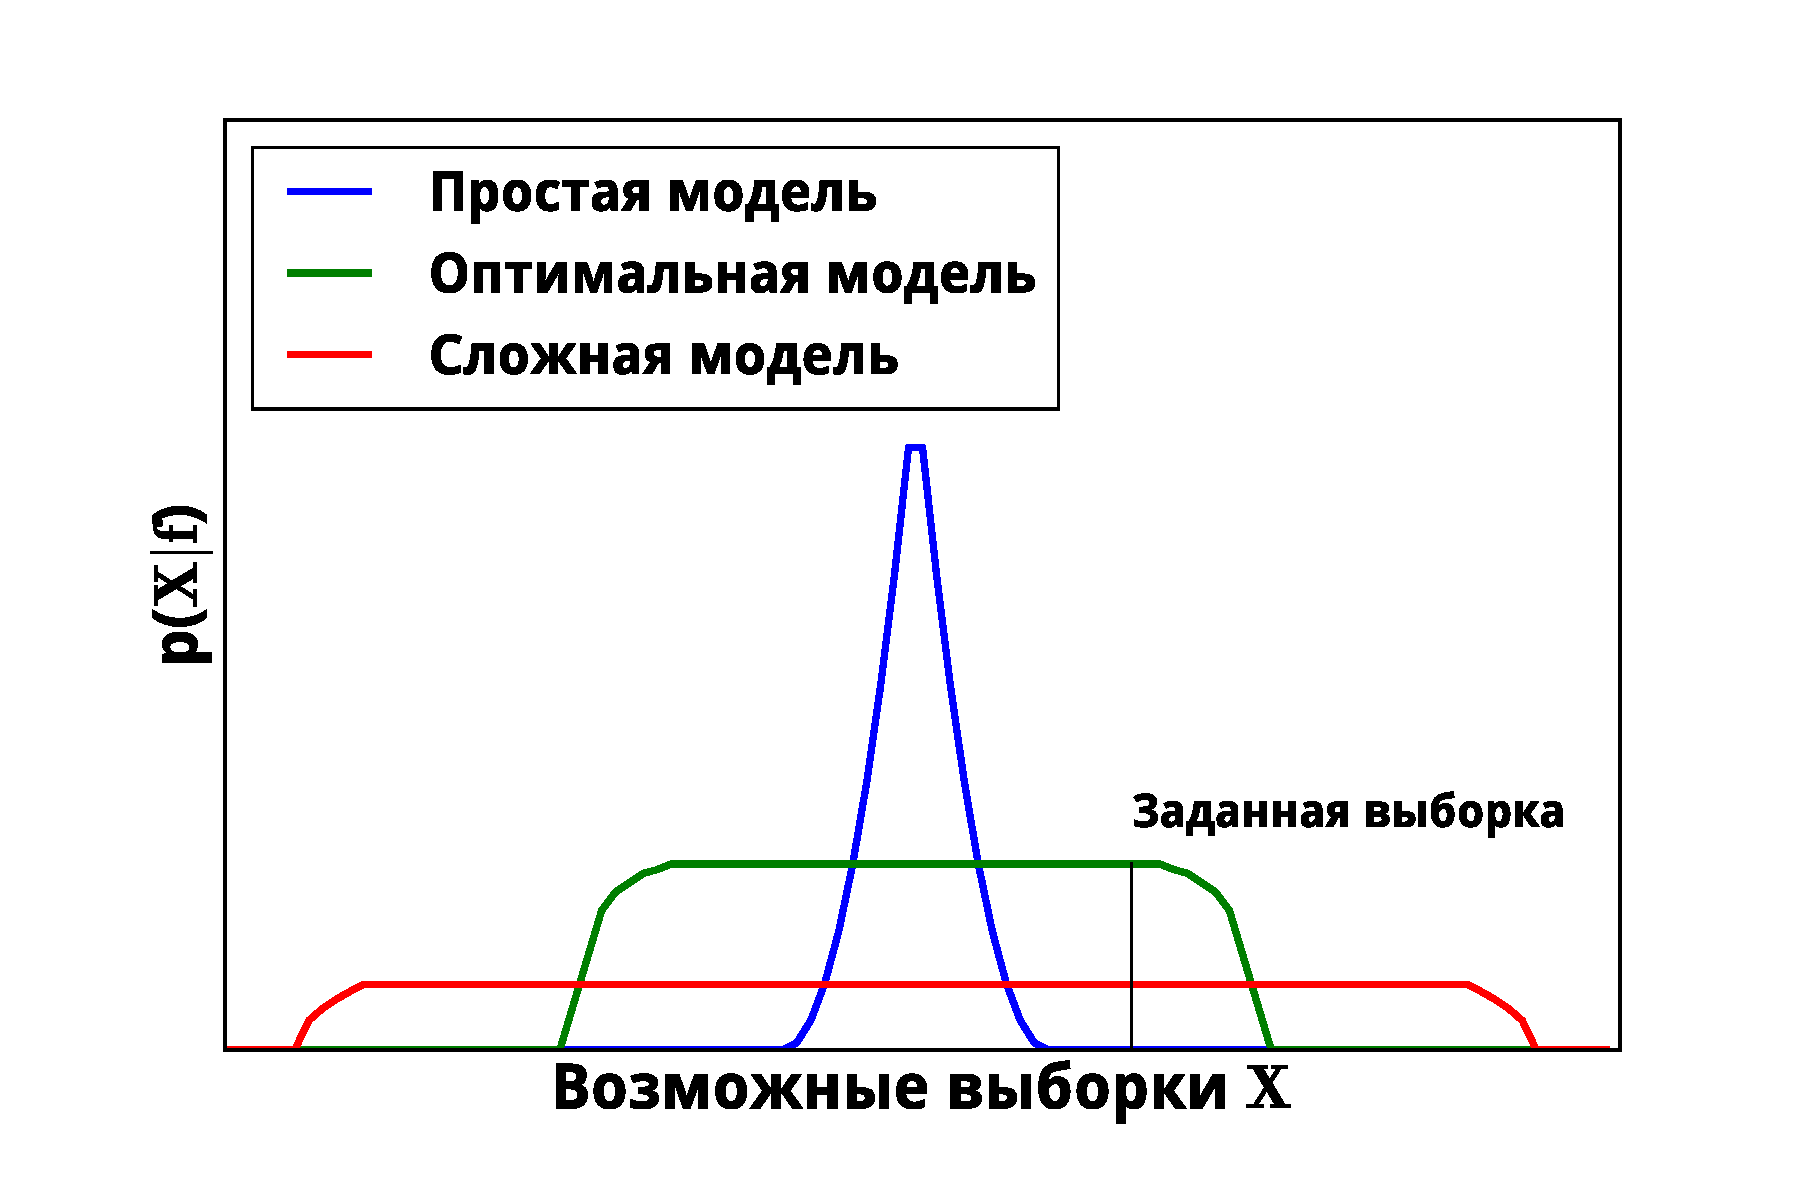
\includegraphics[width=0.45\textwidth]{slide_plots/evidence.pdf}} 
 \subfloat[]{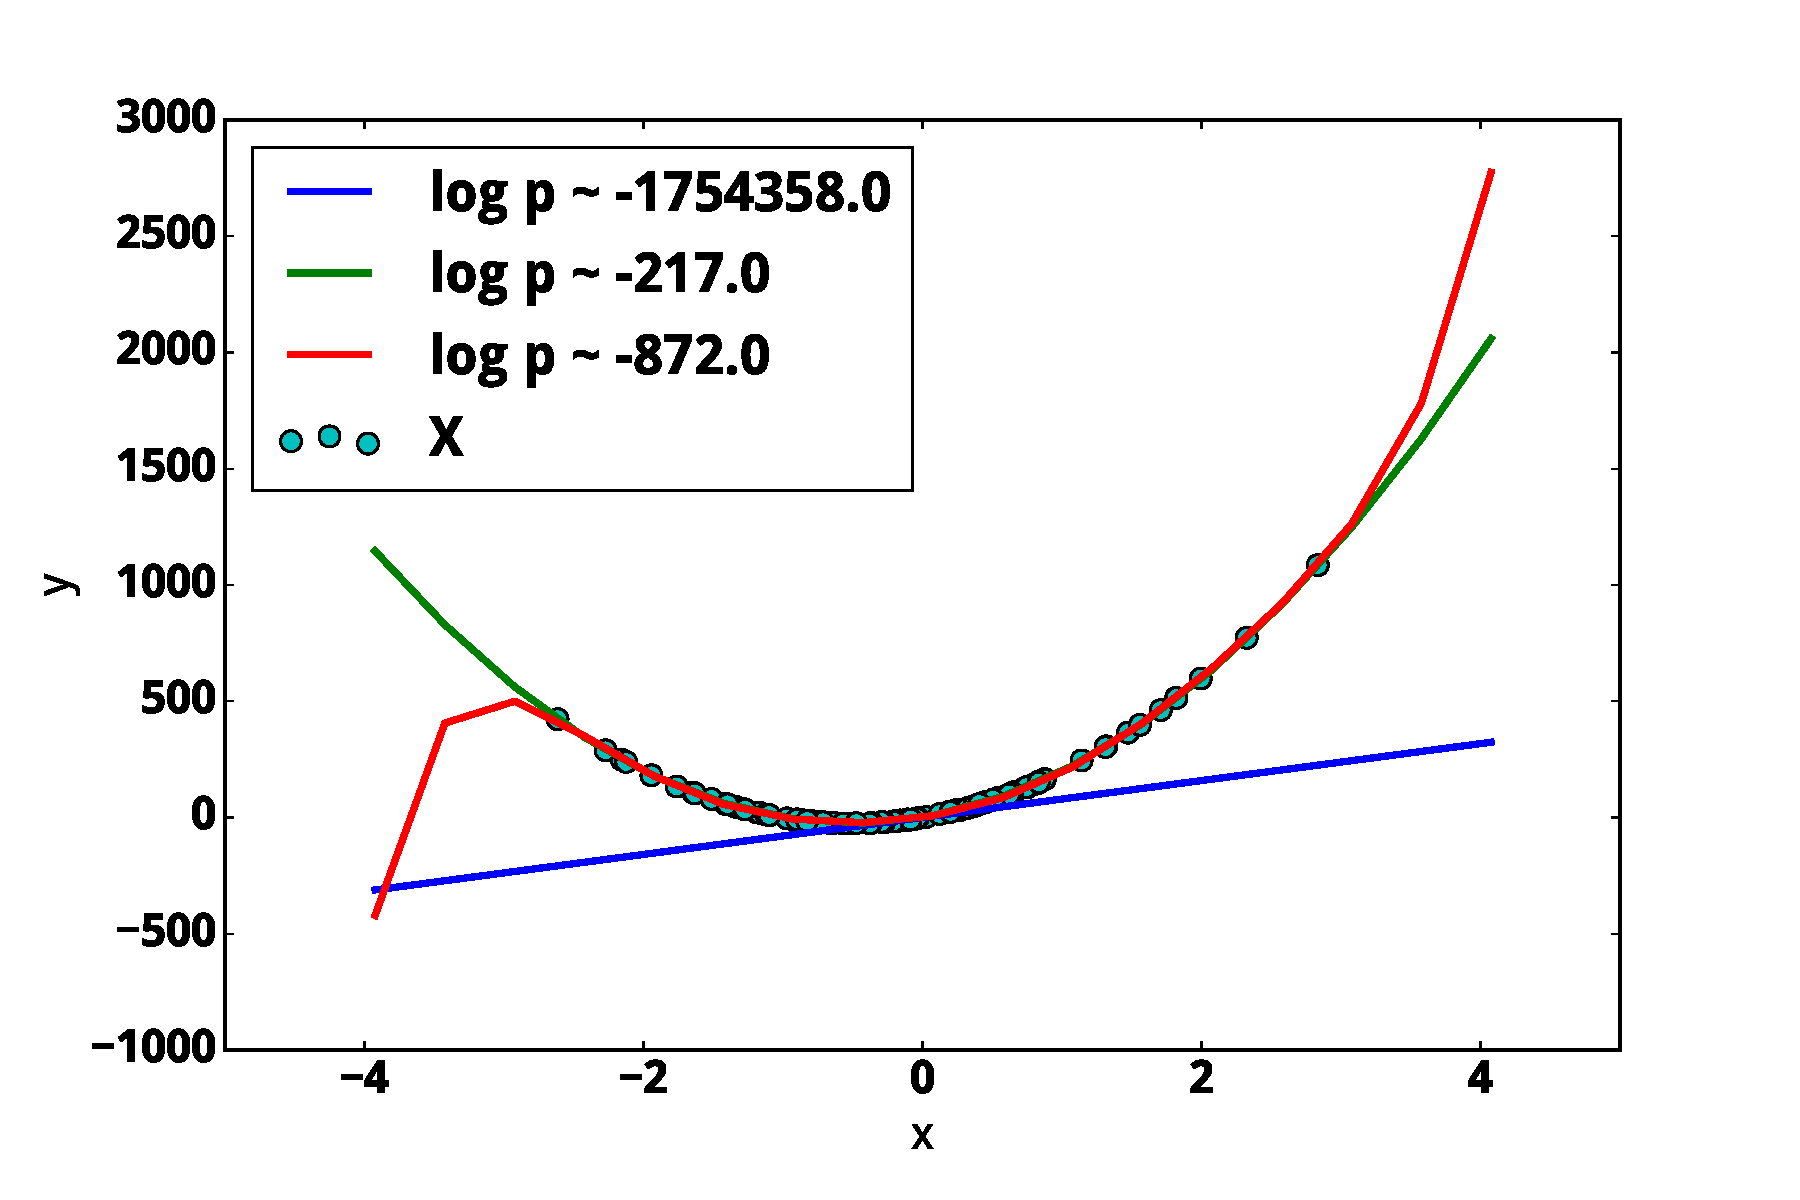
\includegraphics[width=0.45\textwidth]{slide_plots/example.pdf}}

\end{figure}
\end{frame}


\begin{frame}{Вариационная нижняя оценка обоснованности} 
\footnotesize

Интеграл обоснованности невычислим аналитически.\\
\textbf{Обоснованность модели:}
\[
p(\mathbf{y}|\mathbf{X}, \h, \lam) =
 \iint\limits_{\mathbf{w}, \boldsymbol{\Gamma}}  \textcolor{red}{p(\mathbf{y}|\mathbf{X},\mathbf{w},  \boldsymbol{\Gamma})} \textcolor{blue}{p(\mathbf{w}, \boldsymbol{\Gamma}|\h, \lam)}d\mathbf{w}d{\boldsymbol{\Gamma}}.                         
\]

\begin{columns}
\begin{column}{0.55\textwidth}
  
\begin{block}{Определение}
\textit{Вариационными параметрами} модели $\boldsymbol{\theta} \in \Tetab$ назовем параметры распределения $q$, приближающие апостериорное распределение параметров и структуры $p(\mathbf{w}, \boldsymbol{\Gamma}|\mathbf{X}, \mathbf{y}, \mathbf{h}, \lam)$:
\[
    q \approx  \frac{\textcolor{blue}{p(\mathbf{y}|\mathbf{X},\mathbf{w},\boldsymbol{\Gamma})}\textcolor{red}{p(\mathbf{w}, \boldsymbol{\Gamma}|\mathbf{h}, \lam)}}{\iint\limits_{\mathbf{w}', \boldsymbol{\Gamma'}}\textcolor{blue}{p(\mathbf{y}|\mathbf{X},\mathbf{w}',\boldsymbol{\Gamma}')}\textcolor{red}{p(\mathbf{w}', \boldsymbol{\Gamma}'|\mathbf{h}, \lam)}d\mathbf{w}'d\boldsymbol{\Gamma}'}.
\]
\end{block} 

\end{column}
\begin{column}{0.45\textwidth}  %%<--- here
    \begin{center}
     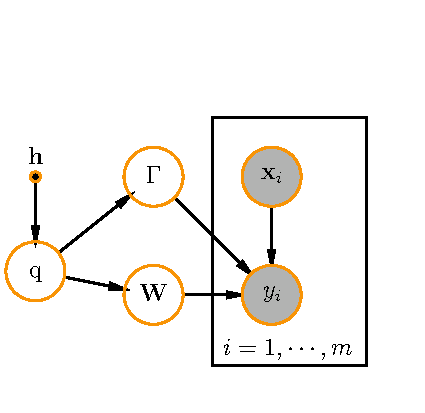
\includegraphics[width=\textwidth]{plate.pdf}
     \end{center}
\end{column}
\end{columns}



%Пусть $q(\mathbf{W}, \boldsymbol{\Gamma}) = q_{\mathbf{W}}(\mathbf{W})q_{\boldsymbol{\Gamma}}(\boldsymbol{\Gamma})$ --- непрерывное распределение, аппроксимирующее 
%апостериорное распределение $p(\mathbf{W}, \boldsymbol{\Gamma}|\mathbf{y}, \mathbf{X})$.
~\\Получим нижнюю оценку $\text{log}\hat{{p}}(\mathbf{y}|\mathbf{X}, \h, \lam)$ интеграла
$$                                                                                                                                              
        \text{log}~p(\mathbf{y}|\mathbf{X}, \h, \lam) \geq 
\textcolor{blue}{\mathsf{E}_q \text{log}~{p(\mathbf{y} | \mathbf{X}, \mathbf{w}, \boldsymbol{\Gamma},\h, \lam)}} - \textcolor{red}{\text{D}_{KL}\bigl(q(\mathbf{w}, \boldsymbol{\Gamma})||p(\mathbf{w}, \boldsymbol{\Gamma}| \h, \lam)\bigr)}.
$$ 



Она совпадает с интегралом обоснованности при $$D_\text{KL}\bigl(q(\mathbf{w}, \boldsymbol{\Gamma})|p\left(\mathbf{w}, \boldsymbol{\Gamma}|\mathbf{y}, \mathbf{X}, \lam, \h\right)\bigr)=0.$$

\end{frame}      


\begin{frame}{Задача выбора модели}
\footnotesize
Зададим вариационное распределение $q=q_\mathbf{w}q_{\boldsymbol{\Gamma}}$ с параметрами $\boldsymbol{\theta}$, приближающие апостериорное распределение $p(\mathbf{w}, \boldsymbol{\Gamma}|\mathbf{X}, \mathbf{y}, \mathbf{h}, \lam)$ параметров и структуры.



\begin{block}{Определение}

\textit{Функцией потерь} $\Loss$   назовем дифференцируемую функцию, качество модели на обучающей выборки при параметрах $\boldsymbol{\theta}$ распределения $q$.~\\~\\
\textit{Функцией валидации} $\Val$ назовем дифференцируемую функцию, качество модели при векторе $\boldsymbol{\theta}$, заданном неявно.
\end{block}
\begin{block}{}
\textit{Задачей выбора модели} $\mathbf{f}$ назовем двухуровневую задачу оптимизации:

\[
	\mathbf{h}^{*} = \argmax_{\mathbf{h} \in \mathbb{H}} \Val[][][][{\teta}^{*}],
\]
где $\boldsymbol{\theta}^{*}$ --- решение задачи оптимизации
\[
   \boldsymbol{\theta}^{*} = \argmax_{\boldsymbol{\theta} \in \Tetab} \Loss.
\]
\end{block}


\end{frame}







                                                                                                              


   
\begin{frame}{Обобщающая задача}
\footnotesize
%\begin{block}{Определение}
Задачу выбора модели $\mathbf{h}^{*}, \boldsymbol{\theta}^{*}$ назовем обобщаюшей на множестве $U_{\theta}\times U_{h} \times U_{\lambda} \subset \mathbb{R}^{u} \times \mathbb{H} \times \amsmathbb{\Lambda}$, если выполнены условия:
\begin{enumerate}
\item Область параметров, гиперпараметров и метапараметров не является пустым или точкой.
\item Для каждого $\mathbf{h} \in U_h$ и каждого $\boldsymbol{\lambda} \in U_{\lambda}$ решение $\boldsymbol{\theta}^{*}$ определено однозначно.


\item \textbf{Критерий непрерывности: } $L, Q$ непрерывны по метапараметрам.
\item \textbf{Критерий \textcolor{OliveGreen}{перехода между структурами: }}
%\textcolor{darkgray}{
существует константа $K_3>0$, такая, что для произвольных локальных оптимумов  $\mathbf{h}_1,\mathbf{h}_2$ задачи оптимизации $Q$, полученных при метапараметрах $\boldsymbol{\lambda}$ и удовлетворяющих неравенствам $$D_\text{KL}\left(p(\boldsymbol{\Gamma}| \mathbf{h}_1, \boldsymbol{\lambda}) | p(\boldsymbol{\Gamma}| \mathbf{h}_1, \boldsymbol{\lambda})\right) > K_3, D_\text{KL}\left(p(\boldsymbol{\Gamma}| \mathbf{h}_1, \boldsymbol{\lambda}) | p(\boldsymbol{\Gamma}| \mathbf{h}_2, \boldsymbol{\lambda})\right) > K_3,$$ $$Q(\mathbf{h}_1|\boldsymbol{\lambda})>Q(\mathbf{h}_2|\boldsymbol{\lambda}),$$  существует значение метапараметров $\boldsymbol{\lambda}' \neq \boldsymbol{\lambda}$, такое, что
\begin{enumerate}
\item соответствие между вариационными параметрами $\boldsymbol{\theta}^{*}(\mathbf{h}_1),\boldsymbol{\theta}^{*}(\mathbf{h}_2)$ сохраняется при  $\boldsymbol{\lambda}'$,
\item выполняется неравенство $Q(\mathbf{h}_1|\boldsymbol{\lambda}')<Q(\mathbf{h}_2|\boldsymbol{\lambda}')$.
\end{enumerate}
%}



\end{enumerate}
%\end{block}
\end{frame}

\begin{frame}{Обобщающая задача}
\footnotesize
%\begin{block}{Определение}
Задачу выбора модели $\mathbf{h}^{*}, \boldsymbol{\theta}^{*}$ назовем обобщаюшей на множестве $U_{\theta}\times U_{h} \times U_{\lambda} \subset \mathbb{R}^{u} \times \mathbb{H} \times \amsmathbb{\Lambda}$, если выполнены условия:
\begin{enumerate}
\setcounter{enumi}{4}
\item \textbf{Критерий \textcolor{blue}{максимизации правдоподобия выборки: }}\textcolor{darkgray}{ существует $\boldsymbol{\lambda} \in U_{\lambda}$ и  $K_1 \in \mathbb{R}_{+}$, такие что для любых векторов гиперпараметров $\mathbf{h}_1, \mathbf{h}_2 \in  U_{h}, Q(\mathbf{h}_1) - Q(\mathbf{h}_2) > K_1:$ выполнено: $\mathsf{E}_{\q[{\teta}^{*}(\h_1)]} \text{log} \LL>\mathsf{E}_{\q[{\teta}^{*}(\h_2)]} \text{log} \LL$.}

% здесь мы имеем ввиду что для любого lambda, такого что мы считаем параметр неинформативными
\item \textbf{Критерий \textcolor{red}{минимизации параметрической сложности модели: }}\textcolor{darkgray}{ существует  $\boldsymbol{\lambda} \in U_{\lambda}$ и $K_2 \in \mathbb{R}_{+}$, такие что для любых векторов гиперпараметров $\mathbf{h}_1, \mathbf{h}_2 \in U_h, Q(\mathbf{h}_1) - Q(\mathbf{h}_2) > K_2$, сложность первой модели меньше, чем второй.}

\item \textbf{Критерий максимизации обоснованности модели: }\textcolor{darkgray}{ существует значение гиперпараметров $\boldsymbol{\lambda}$, такое что оптимизация задачи эквивалента оптимизации вариационной оценки обоснованности модели:
\vspace{-0.2cm}
\[
    \mathbf{h}^{*} \propto \argmax_{} \E_{\q} \log  \LL - \KL{\q}{\prior} + \log p(\mathbf{h}|\boldsymbol{\lambda}),
\]
\[
    \boldsymbol{\theta}^{*} = \argmin D_\text{KL}(q| p(\mathbf{w}, \boldsymbol{\Gamma}|\mathbf{y}, \mathbf{X}, \h, \lam)).
\]}
\vspace{-0.6cm}
\end{enumerate}
%\end{block}
\end{frame}

\begin{frame}{Анализ задач выбора моделей}
\small
\begin{block}{Теорема [Бахтеев, 2019]}
Следующие задачи выбора модели не являются обобщающими:
\begin{enumerate}
% задача не является строго двууровневой, нельзя проомтимизировать ELBO
\item критерий максимума правдоподобия: $\max_{\boldsymbol{\theta}} \textcolor{blue}{\mathsf{E}_q \text{log} p(\mathbf{y}|\mathbf{X}, \boldsymbol{\theta}, \lambda_\text{temp}, \mathbf{f})};$

% нет возможности оптимизации структуры
\item критерий максимума апостериорной вероятности $\max_{\boldsymbol{\theta}} \textcolor{blue}{\mathsf{E}_q \text{log} p(\mathbf{y}|\mathbf{X},  \boldsymbol{\theta}, \mathbf{f})}\textcolor{red}{p( \boldsymbol{\theta}| \mathbf{h}, \lambda_\text{temp})};$

% нет возможности оптимизации правдоподобия модели - структа не подчиняется beta
\item метод максимума вариационной оценки обоснованности модели $\max_{\mathbf{h}} \max_{\boldsymbol{\theta}} \textcolor{blue}{\mathsf{E}_q \text{log}~{p(\mathbf{y} | \mathbf{X}, \mathbf{w}, \boldsymbol{\Gamma}, \mathbf{f})}} - \textcolor{red}{\text{D}_{KL}\bigl(q(\mathbf{w}, \boldsymbol{\Gamma})||p(\mathbf{w}, \boldsymbol{\Gamma}, \lambda_\text{temp})\bigr)} + \textcolor{OliveGreen}{\text{log}~p(\mathbf{h}|\mathbf{f})};$

\item кросс-валидация $\max_{\mathbf{h}} \textcolor{blue}{\mathsf{E}_q \text{log}p(\mathbf{y}_\text{valid}|\mathbf{X}_\text{valid}, \boldsymbol{\theta}^{*}, \lambda_\text{temp}, \mathbf{f})}$, $\boldsymbol{\theta}^{*} = \argmax_{\boldsymbol{\theta}} \textcolor{blue}{\mathsf{E}_q \text{log}p(\mathbf{y}_\text{train}|\mathbf{X}_\text{train}, \boldsymbol{\theta}, \lambda_\text{temp}, \mathbf{f})}\textcolor{red}{p(\boldsymbol{\theta}| \mathbf{h})}$.

% задача не является строго двууровневой, нельзя проомтимизировать ELBO
\item AIC: $\max_{\boldsymbol{\theta}} \textcolor{blue}{\mathsf{E}_q \text{log} p(\mathbf{y}|\mathbf{X}, \boldsymbol{\theta}, \lambda_\text{temp}, \mathbf{f})} - \textcolor{red}{|\theta_i: \text{D}_\text{KL}\left(q(w_i)|p(w_i|\boldsymbol{\Gamma}, \mathbf{h}, \boldsymbol{\lambda}\right) < \lambda|}$;

% задача не является строго двууровневой, нельзя проомтимизировать ELBO
\item BIC: $\max_{\boldsymbol{\theta}} \textcolor{blue}{\mathsf{E}_q \text{log} p(\mathbf{y}|\mathbf{X}, \boldsymbol{\theta}, \lambda_\text{temp}, \mathbf{f})} - \textcolor{red}{\frac{1}{2}\text{log}(|\mathbb{W}|{|\theta_i: \text{D}_\text{KL}\left(q(w_i)|p(w_i|\boldsymbol{\Gamma}, \mathbf{h}, \boldsymbol{\lambda}\right) < \lambda|}}$;


\item перебор структуры модели:   $\max{\boldsymbol{\Gamma}'} \max_{\boldsymbol{\theta}} \textcolor{blue}{\mathsf{E}_q \text{log} p(\mathbf{y}|\mathbf{X}, \boldsymbol{\theta}, \lambda_\text{temp}, \mathbf{f})}\textcolor{red}{\mathbb{I}(q(\boldsymbol{\Gamma}{\Gamma} = p') },$ где $p'$ --- распределение на структуре (метапараметр).
\end{enumerate}
\end{block}
\end{frame}

\begin{frame}{Предлагаемая задача оптимизации}

\footnotesize
\begin{columns}
\begin{column}{0.8\textwidth}
\begin{block}{Теорема [Бахтеев, 2018]}
Тогда следующая задача является обобщающей:
\[
\mathbf{h}^{*} = \argmax_{\mathbf{h}} Q = 
\]
\[
= \textcolor{blue}{\lamLL\mathsf{E}_{\q[\teta^{*}]} \text{log}~{p(\mathbf{y} | \mathbf{X}, \mathbf{w},\boldsymbol{\Gamma}, \mathbf{h}, \lam)}}
 -\]
\vspace{-0.3cm}
\[- \textcolor{red}{^\text{prior}_\text{Q}\text{D}_{KL}\bigl(\q[\teta^{*}] || p(\mathbf{w}, \boldsymbol{\Gamma} |\mathbf{h}, \lam) \bigr)}  -\]
\vspace{-0.3cm}
\[
 - \textcolor{OliveGreen}{\sum_{p' \in \mathfrak{P}, \lambda \in \boldsymbol{\lambda}^\text{struct}_\text{Q}} \lambda\text{D}_{KL}(\priorG | p') + \text{log}p(\mathbf{h}|\lam)}, 
\]
где 
\[
\teta^{*} = \argmax_{\teta} L = 
\textcolor{blue}{\mathsf{E}_q \text{log}~{p(\mathbf{y} | \mathbf{X}, \mathbf{w}, \boldsymbol{\Gamma}, \mathbf{h}, \lam)}}
\]
\vspace{-0.3cm}
\[- \textcolor{red}{^\text{prior}_\text{L}\text{D}_{KL}\bigl( q^{*}(\mathbf{w}, \boldsymbol{\Gamma}) || p(\mathbf{w}, \boldsymbol{\Gamma} |\mathbf{h}, \lam) \bigr)}.
\]
\end{block}
%$\lambda^\text{likelihood}_\text{L}, \lambda^\text{prior}_\text{L}, \lambda^\text{prior}_\text{Q},  \boldsymbol{\lambda}_{\text{struct}}^Q, \lambda_{\text{temp}}$ и параметры распределений $\mathbf{P}$ --- метапараметры оптимизации.\\
Оптимизационная задача обобщает алгоритмы оптимизации: оптимизация правдоподобия и обоснованности, последовательное увеличение и снижение сложности модели, полный перебор структуры.
\end{column}
\begin{column}{0.2\textwidth}
\begin{figure}
\centering
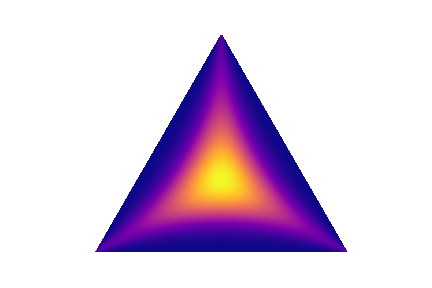
\includegraphics[width=0.75\textwidth]{combinations_1.png}
\end{figure}
\vspace{-0.2cm}
$ \textcolor{OliveGreen}{\boldsymbol{\lambda}_{\text{struct}}^Q=[0;0;0].}$
\begin{figure}
\centering
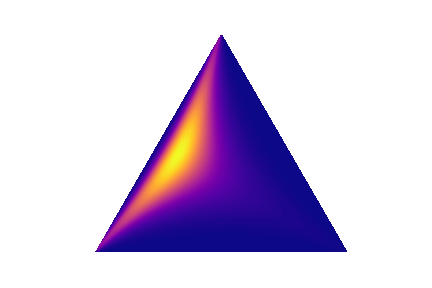
\includegraphics[width=0.75\textwidth]{combinations_2.png}
\end{figure}
\vspace{-0.2cm}
$ \textcolor{OliveGreen}{\boldsymbol{\lambda}_{\text{struct}}^Q=[1;0;0].}$
\begin{figure}
\centering
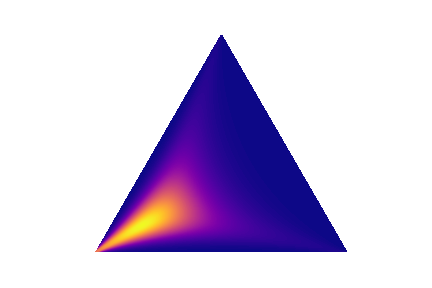
\includegraphics[width=0.75\textwidth]{combinations_3.png}
\end{figure}
\vspace{-0.2cm}
$ \textcolor{OliveGreen}{\boldsymbol{\lambda}_{\text{struct}}^Q=[1;1;0].}$
\end{column}
\end{columns}
\end{frame}


\begin{frame}{Адекватность задачи оптимизации}
\footnotesize
\begin{block}{Теорема, [Бахтеев, 2018]}
Пусть задано параметрическое множество вариационных распределений: $q(\boldsymbol{\theta})$. 
Пусть $\textcolor{blue}{\lambda^L_\text{likelihood}} = \textcolor{red}{\lambda^L_\text{prior}=\lambda^Q_\text{prior}}=1, \textcolor{OliveGreen}{\boldsymbol{\lambda}^Q_{\text{struct}}}=\mathbf{0}$. Тогда:
\begin{enumerate}
\item Предлагаемая задача оптимизации доставляет максимум апостериорной вероятности гиперпараметров с использованием вариационной оценки обоснованности:
\vspace{-0.3cm}
\[
    \text{log}\hat{p}(\mathbf{y}|\mathbf{X}, \mathbf{h}, \lam) + \textcolor{OliveGreen}{\text{log}p(\mathbf{h}|\lam)} \to \max_{\mathbf{h}}.
\]
\item Вариационное распределение $q$ приближает апостериорное распределение $p(\mathbf{w}, \boldsymbol{\Gamma}|\mathbf{y}, \mathbf{X}, \mathbf{h}, \lam, \mathbf{f})$ наилучшим образом:
\vspace{-0.3cm}
\[
    {D}_\text{KL}(q||p(\mathbf{w}, \boldsymbol{\Gamma}|\mathbf{y}, \mathbf{X}, \mathbf{h}, \lam)) \to \min_{\boldsymbol{\theta}}.
\]
\end{enumerate}
\end{block}
% proof
% 1. по определению
% 2. тоже по определению
\begin{block}{}
Пусть также распределение $q$ декомпозируется на два независимых распределения для параметров $\mathbf{w}$ и структуры $\boldsymbol{\Gamma}$ модели $\mathbf{f}$:
\[
    q = q_{\mathbf{w}}q_{\boldsymbol{\Gamma}}, q_{\boldsymbol{\Gamma}} \approx p(\boldsymbol{\Gamma}|\mathbf{y}, \mathbf{X}, \mathbf{h}, \lam), q_{\mathbf{w}} \approx p(\mathbf{w}|\boldsymbol{\Gamma},\mathbf{y}, \mathbf{X}, \mathbf{h}, \lam).
\]
Если существуют значения вариационных параметров, такие что $q(\mathbf{w}) = p(\mathbf{w}| \boldsymbol{\Gamma}, \mathbf{h}, \lam),$ $q(\boldsymbol{\Gamma}) = p(\boldsymbol{\Gamma}| \mathbf{h}, \boldsymbol{\lambda}),$
то решение задачи оптимизации для функции $L$ доставляет эти значения.
\end{block}
%http://akosiorek.github.io/ml/2017/09/10/kl-hierarchical-vae.html. Важно: D_KL во втором случае - условная
% декомпозируем на два D_KL
% обе D_KL независимы как функции, поэтому ок, можем минимизировать
\end{frame}





\begin{frame}{Оператор оптимизации}
\small
\begin{block}{Определение}
Назовем \textit{оператором оптимизации}  $T$ выбор вектора параметров $\boldsymbol{\theta}'$  по параметрам предыдущего шага $\boldsymbol{\theta}$.
\end{block}
Оператор стохастического градиентного спуска:
\[
	 \hat{\boldsymbol{\theta}} = T \circ T \circ \dots \circ T(\boldsymbol{\theta}_0, \mathbf{h}) = T^\eta(\boldsymbol{\theta}_0, \mathbf{h}), \quad\text{где}	T(\boldsymbol{\theta}, \mathbf{h}) =
\]
\[=\boldsymbol{\theta} - \lambda_\text{lr} \nabla \left(-L(\boldsymbol{\theta}, \mathbf{h})|_{\hat{\mathfrak{D}}}\right), 
\]
$\lambda_{\text{lr}}$ --- длина шага градиентного спуска, $\boldsymbol{\theta}_0$ --- начальное значение параметров $\boldsymbol{\theta}$, $\hat{\mathfrak{D}}$ --- случайная подвыборка исходной выборки $\mathfrak{D}$.


Перепишем итоговую задачу оптимизации:
\[
	 \mathbf{h}' = T^\eta\bigl(Q, \mathbf{h}, T^\eta(L, \boldsymbol{\theta}_0, \mathbf{h})\bigr),
\]
где $\boldsymbol{\theta}_0$ --- начальное значение $\boldsymbol{\theta}$.

\begin{block}{Теорема, [Бахтеев, 2019]}
Пусть $\frac{\lambda^Q_\text{prior}}{\lambda^Q_\text{likelihood}} = {\lambda^L_\text{prior}}.$ Тогда задача оптимизации представима в виде одноуровневой задач.
\end{block}

\end{frame}



\begin{frame}
\small
\frametitle{Нижняя вариационная оценка обоснованности на основе мультистарта}
$$\text{log}p(\mathbf{y}|\mathbf{X}, \mathbf{h},\lam) \geq \mathsf{E}_{q(\mathbf{W)}}\text{log~}p (\mathbf{y}, \mathbf{w}|\mathbf{X}, \mathbf{h},\lam) - \mathsf{E}_{q_{\mathbf{w}}}(-\text{log}(q_\mathbf{w})).$$

\begin{block}{Теорема [Бахтеев, 2016]}Пусть $L$ --- функция потерь, градиент которой ---  непрерывно-дифференцируемая функция с константой Липшица $C$. \\
Пусть $\boldsymbol{\theta} = [\mathbf{w}^1,\dots,\mathbf{w}^k]$ ---  начальные приближения оптимизации модели, $\lambda_\text{lr}$ --- шаг градиентного спуска.

Тогда разность энтропий на смежных шагах оптимизации приближается следующим образом:
\small
\[
	\mathsf{E}_{q^{\tau}_{\mathbf{w}}}(-\text{log}(q^{\tau}_\mathbf{w})) -  \mathsf{E}_{q^{\tau-1}_{\mathbf{w}}}(-\text{log}(q^{\tau-1}_\mathbf{w}))  \approx  \frac{1}{k}\sum_{r=1}^k \bigl(\lambda_\text{lr} Tr[\mathbf{H}(\mathbf{w}^r)] - \lambda_\text{lr}^2 Tr[\mathbf{H}(\mathbf{w}^r)\mathbf{H}(\mathbf{w}^r)]  \bigr),
\]
где $\mathbf{H}$ --- гессиан минус функции потерь $-L$, $q^{\tau}_\mathbf{w}$ --- распределение $q^{\tau}_\mathbf{w}$ в момент оптимизации $\tau$.
\end{block}
\end{frame}



\begin{frame}

\frametitle{Градиентный спуск как вариационная оценка обоснованности модели}
\footnotesize
Эмпирическое распределение на точках старта оптимизации --- вариационное распределение.\\


\begin{multicols}{2}
Градиентный спуск не оптимизирует оценку обоснованности.
\vspace{-1.cm}
\begin{figure}

\subfloat{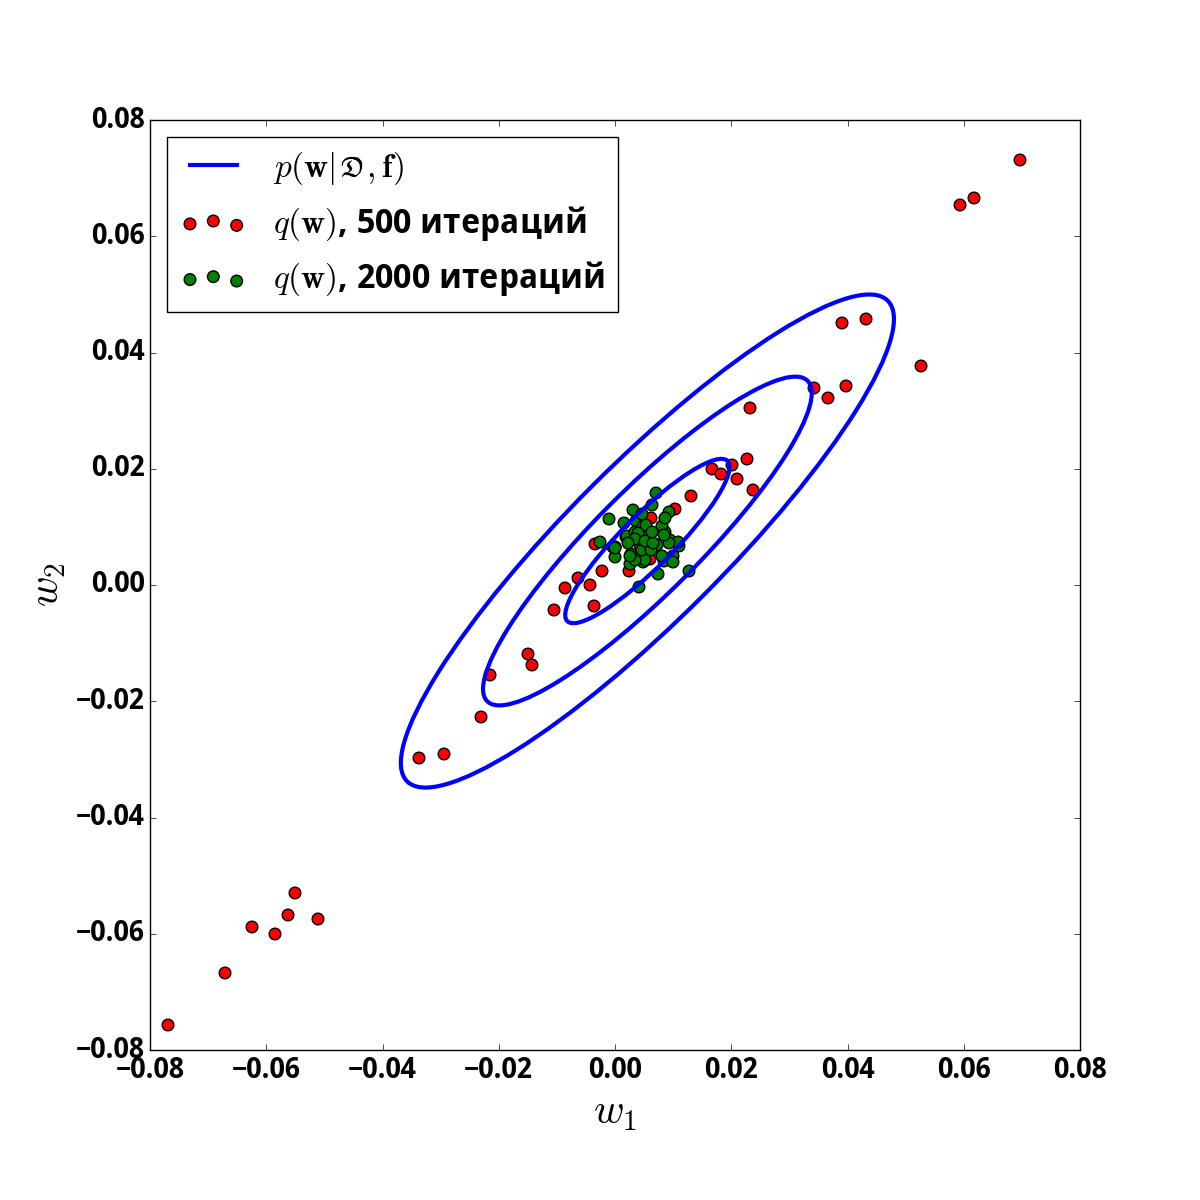
\includegraphics[width=0.52\textwidth]{./slide_plots/sgd_estimate.png}}
\end{figure}

\columnbreak

Снижение вариационной оценки обоснованности ---  начало переобучения.
\vspace{-1.2cm}
\begin{figure}
{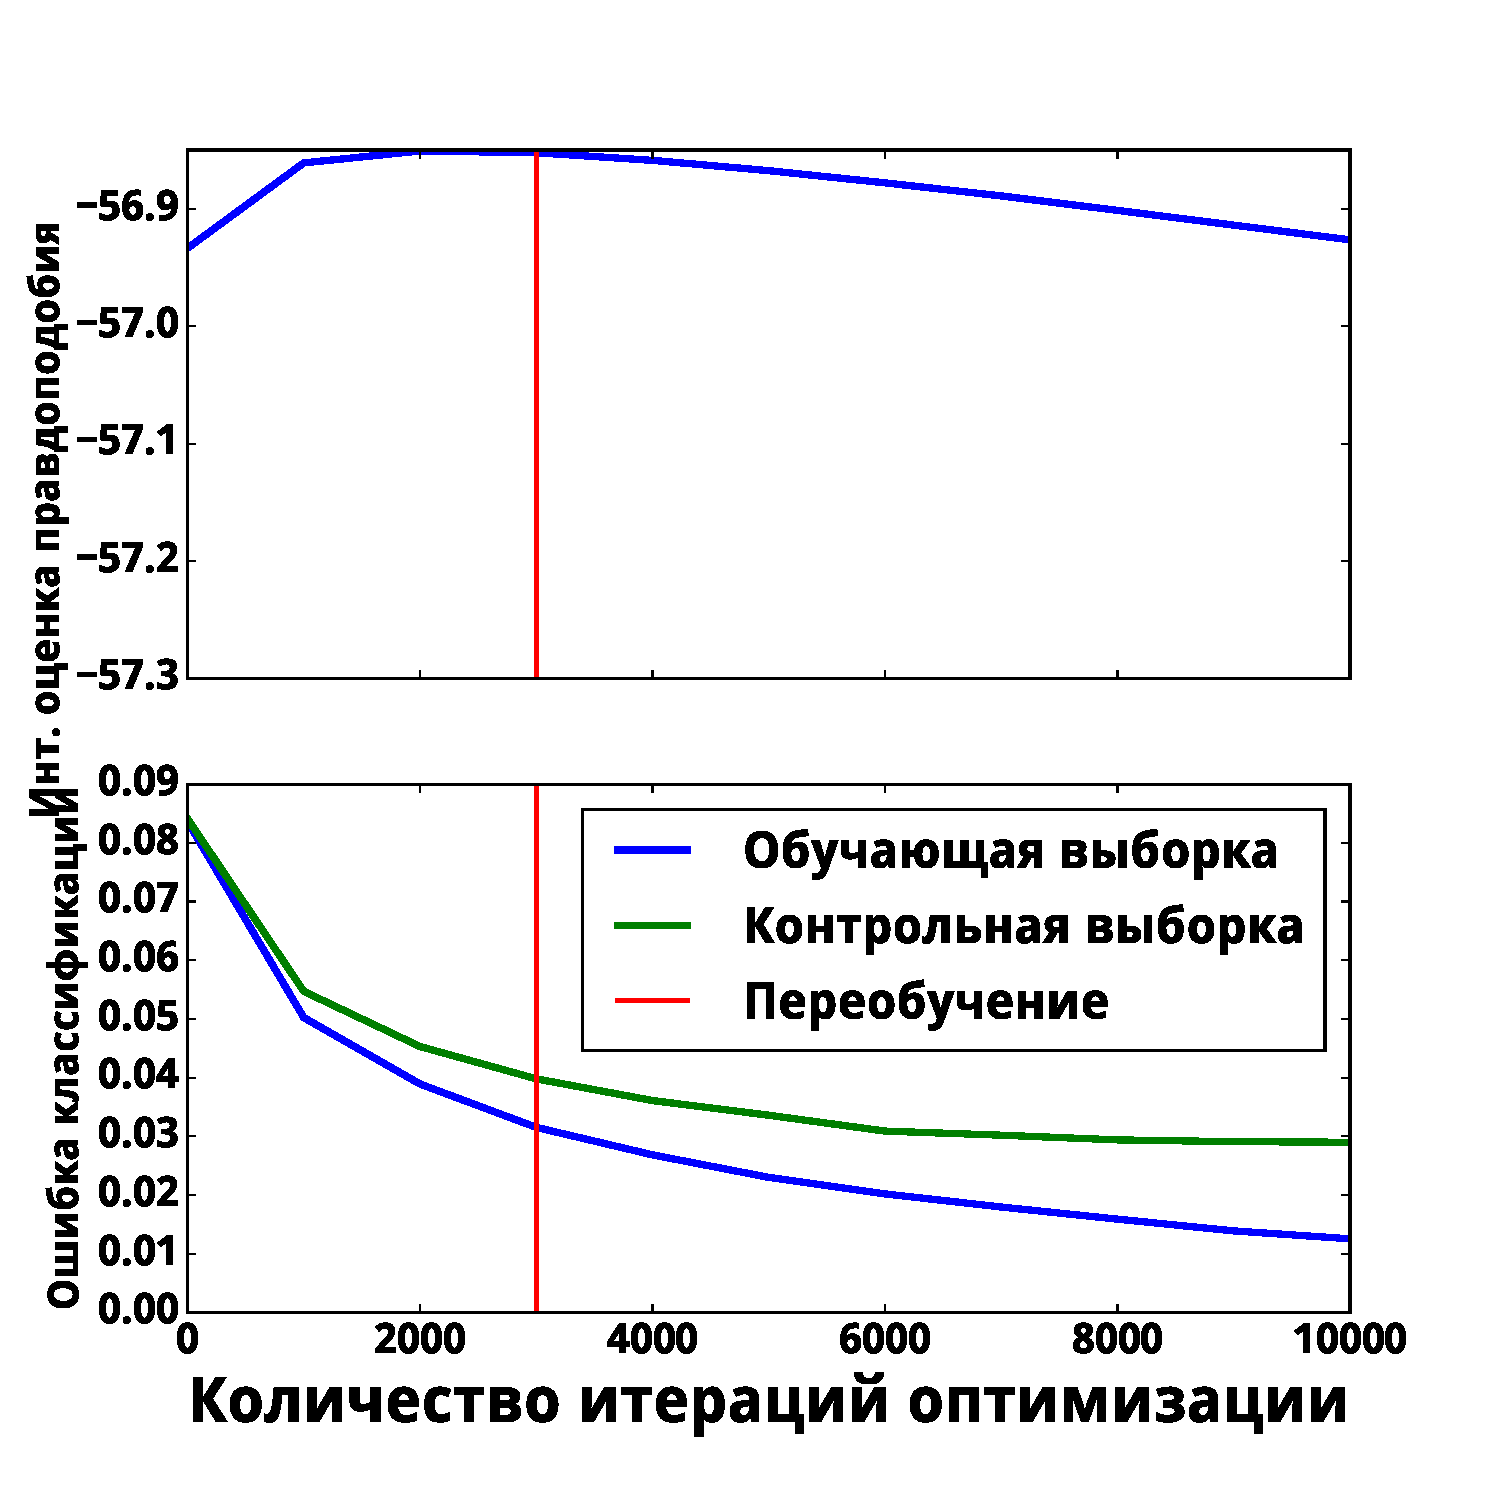
\includegraphics[width=0.52\textwidth]{./slide_plots/sgd_show.pdf}}
\end{figure}
\end{multicols}
\end{frame}










\begin{frame}{Анализ обобщающей задачи оптимизации}
\footnotesize

\vspace{-0.1cm}
\begin{block}{Теорема, [Бахтеев, 2018]}
Пусть $\textcolor{red}{\lambda_\text{prior}^L} > 0, m \gg 0, \frac{m}{\lambda_\text{prior}^L} \in \mathbb{N}.$ Тогда оптимизация функции\vspace{-0.3cm} \[L = 
\textcolor{blue}{\mathsf{E}_q \text{log}~{p(\mathbf{y} | \mathbf{X}, \mathbf{w}, \boldsymbol{\Gamma})}} - \textcolor{red}{\lambda_\text{prior}^L\text{D}_{KL}(q||p(\mathbf{w}, \boldsymbol{\Gamma} |\mathbf{h}, \lam)}\vspace{-0.2cm}\] эквивалентна минимизации $\mathsf{E}_{\hat{\mathbf{X}}, \hat{\mathbf{y}}\sim p(\mathbf{X}, \mathbf{y})}\text{D}_{KL}(q||p(\mathbf{w}, \boldsymbol{\Gamma} | \hat{\mathbf{X}}, \hat{\mathbf{y}},\mathbf{h},\lam)),$ где $\hat{\mathbf{X}}, \hat{\mathbf{y}}$ --- случайные подвыборки мощностью $\frac{m}{\textcolor{red}{\lambda_\text{prior}^L}}$ из генеральной совопкупности.
\end{block}
\vspace{-0.2cm} 
\begin{block}{Определение}
Параметрической сложностью модели назовем минимальную дивергенцию между априорным и вариационным распределением:
\vspace{-0.2cm}
\[
    C_p = \min_{\mathbf{h}} \textcolor{red}{D_\text{KL}(q||p(\mathbf{w}, \boldsymbol{\Gamma}|\mathbf{h},\lam)).}
\]
\end{block}
\vspace{-0.2cm}
\begin{block}{Теорема, [Бахтеев, 2018]}
Пусть $\textcolor{OliveGreen}{\boldsymbol{\lambda}^Q_{\text{struct}}} = \bf 0$.
Пусть  $\teta_1, \teta_2, \h_1, \h_2$ --- результаты оптимизации при разных значениях гиперпараметров $\textcolor{red}{{\lamCQ}_1,{\lamCQ}_2, {\lamCQ}_1>{\lamCQ}_2}$ на компакте $U$.
Пусть функция $\Val$ является вогнутой на $U$ при $\textcolor{red}{{\lamCQ}_2}$.
Тогда:
\footnotesize
\vspace{-0.2cm}
\[
    C_p(\teta_1|\Uh, \lam_1) - C_p(\teta_2|\Uh, \lam_2)  < \frac{\lamCL }{{\lamCQ}_2} ({\lamCQ}_2- \lamCL) C,
\]
где $C$ --- некоторая константа.
\end{block}



\end{frame}




\begin{frame}{Анализ параметрической сложности}


\vspace{-0.2cm} 
\begin{block}{Определение}
Относительной вариационной   плотностью  назовем отношение:
\[
\rho(w|\boldsymbol{\Gamma},\boldsymbol{\theta}_\mathbf{w}, \mathbf{h},\boldsymbol{\lambda})=\frac{q_\mathbf{w}(\text{mode}~p(\mathbf{w}|\boldsymbol{\Gamma}, \mathbf{h}, \boldsymbol{\lambda}))}{q_\mathbf{w}(\text{mode}~{q_\mathbf{w}})}.
\]
\end{block}
\vspace{-0.2cm} 
\begin{block}{Теорема, [Бахтеев, 2018]}
Пусть заданы компактные множества $\Uh \subset \Hb, \Utetaw \subset \Tetawb, \UtetaG \subset \TetaGb$,
вариационное и априорное распределение $\qw$, $\priorw$  являются абсолютно непрерывным и унимодальным на  $U_{\boldsymbol{\theta}}$ с совпадающей модой и матожиданием.
Пусть  мода и матожидание априорного распределения не зависят от гиперпараметров $\h$  и структуры $\Gam$.\\
Пусть задана  бесконечная последовательность векторов вариационных параметров $\teta[1],\teta[2],\dots,\teta[i],\dots \in \Uteta$, такая, что $\lim_{i \to \infty}C_p(\teta[i]|\Uh,\lam) = 0.$
Тогда:
\footnotesize
$$
   \lim_{i \to \infty} \E_{\qG[][{\tetaG[i]}]} {\rho}(\w|\Gam, {\tetaw[i]}, {\h[i]}, \lam)^{-1} = 1, \h[i] = \argmin \KL{\q[\teta_i]}{\prior}.
$$
\end{block}



\end{frame}



\begin{frame}{Результаты, выносимые на защиту}
\footnotesize
\begin{enumerate}
\item Предложен метод байесовского выбора субоптимальной структуры модели глубокого обучения с использованием автоматического определения релевантности параметров.
\item Предложены критерии оптимальной и субоптимальной сложности модели глубокого обучения.
\item Предложен метод графового описания моделей глубокого обучения.
\item Предложено обобщение задачи оптимизации структуры модели, включающее ранее описанные методы выбора модели:
\begin{itemize}
\footnotesize
\item оптимизация обоснованности;
\item последовательное увеличение сложности модели;
\item последовательное снижение сложности модели;
\item полный перебор вариантов структуры модели.
\end{itemize}


\item Предложен метод оптимизации вариационной оценки обоснованности на основе мультистарта оптимизации модели.
\item Предложен алгоритм оптимизации параметров, гиперпараметров и структурных
параметров моделей глубокого обучения.
 
\item Исследованы свойства оптимизационной задачи при различных значениях метапараметров.  Рассмотрены ее асимптотические свойства.

%\item Проведен вычислительный эксперимент, иллюстрирующий работу предложенного метода.

\end{enumerate}
\end{frame}



\begin{frame}{Список работ автора по теме диссертации}
\tiny
\textbf{Публикации ВАК}
\begin{enumerate}
\item Bakhteev, O., Kuznetsova, R., Romanov, A. and Khritankov, A. A monolingual approach to detection of text reuse in Russian-English collection // In 2015 Artificial Intelligence and Natural Language and Information Extraction, Social Media and Web Search FRUCT Conference (AINL-ISMW FRUCT) (pp. 3-10). IEEE. 2015.

\item Бахтеев О.Ю., Попова М.С., Стрижов В.В. Системы и средства глубокого обучения в задачах классификации // Системы и средства информатики. 2016. № 26.2. С. 4-22.
\item Romanov, A., Kuznetsova, R., Bakhteev, O. and Khritankov, A. Machine-Translated Text Detection in a Collection of Russian Scientific Papers. // Computational Linguistics and Intellectual Technologies. 2016. 
\item Bakhteev, O. and Khazov, A., Author Masking using Sequence-to-Sequence Models // In CLEF (Working Notes). 2017.
\item Бахтеев О.Ю., Стрижов В.В. Выбор моделей глубокого обучения субоптимальной сложности // Автоматика и телемеханика. 2018. №8. С. 129-147.
\item Огальцов А.В., Бахтеев О.Ю. Автоматическое извлечение метаданных из научных PDF-документов // Информатика и её применения. 2018.
\item Смердов А.Н., Бахтеев О.Ю., Стрижов В.В. Выбор оптимальной модели рекуррентной сети в задачах поиска парафраза // Информатика и ее применения. 2019.
\item Грабовой А.В., Бахтеев О.Ю., Стрижов В.В. Определение релевантности параметров нейросети // Информатика и её применения. 2019.
\item Bakhteev O., Strijov V. Comprehensive analysis of gradient-based hyperparameter optimization algorithms // Annals of Operations Research. 2019.
\end{enumerate}
\textbf{Выступления с докладом}
\begin{enumerate}
\item ``Восстановление панельной матрицы и ранжирующей модели в разнородных шкалах'', Всероссийская конеренция <<57-я научная конеренция МФТИ>>, 2014.
\item ``Выбор модели глубокого обучения субоптимальной сложности с использованием вариационной оценки правдоподобия'', Международная конференция <<Интеллектуализация обработки информации>>, 2016.
\item ``Градиентные методы оптимизации гиперпараметров моделей глубокого обучения'', Всероссийская конференция <<Математические методы распознавания образов ММРО>>, 2017.
\item ``Детектирование переводных заимствований в текстах научных статей из журналов, входящих в РИНЦ'', Всероссийская конференция <<Математические методы распознавания образов ММРО>>, 2017.
\item ``Байесовский выбор наиболее правдоподобной структуры модели глубокого обучения'', Международная конференция <<Интеллектуализация обработки информации>>, 2018.
\end{enumerate}
\end{frame}



\end{document}
